\chapter{The Real and Complex Number Systems}

\section{Integers}

\subsection*{Definitions and Theorems for Integers}

\begin{definition}[Prime Number]
A positive integer $p > 1$ is prime if its only positive divisors are $1$ and $p$ itself.
\end{definition}

\begin{definition}[Factorial]
For a positive integer $n$, the factorial $n!$ is defined as $n! = n \cdot (n-1) \cdot (n-2) \cdots 2 \cdot 1$.
\end{definition}

\begin{theorem}[Fundamental Theorem of Arithmetic]
Every positive integer greater than $1$ can be written uniquely as a product of prime numbers, up to the order of the factors.
\end{theorem}

\begin{theorem}[Euclid's Theorem on Primes]
There are infinitely many prime numbers.
\end{theorem}

\begin{definition}[Mersenne Prime]
A prime number of the form $2^p - 1$, where $p$ is prime, is called a Mersenne prime.
\end{definition}

\begin{definition}[Fermat Prime]
A prime number of the form $2^{2^n} + 1$ is called a Fermat prime.
\end{definition}

\begin{definition}[Fibonacci Sequence]
The Fibonacci sequence is defined by the recurrence relation $F_{n+1} = F_n + F_{n-1}$ with initial conditions $F_1 = F_2 = 1$.
\end{definition}

\begin{theorem}[Well-Ordering Principle]
Every nonempty set of positive integers contains a smallest member.
\end{theorem}

\begin{theorem}[Mathematical Induction]
Let $P(n)$ be a statement about the positive integer $n$. If:
\begin{enumerate}
\item $P(1)$ is true (base case)
\item For every positive integer $k$, if $P(k)$ is true, then $P(k+1)$ is true (inductive step)
\end{enumerate}
Then $P(n)$ is true for all positive integers $n$.
\end{theorem}

\begin{theorem}[Strong Induction]
Let $P(n)$ be a statement about the positive integer $n$. If:
\begin{enumerate}
\item $P(1)$ is true (base case)
\item For every positive integer $k$, if $P(1), P(2), \ldots, P(k)$ are all true, then $P(k+1)$ is true (strong inductive step)
\end{enumerate}
Then $P(n)$ is true for all positive integers $n$.
\end{theorem}



\begin{problembox}[1.1: No Largest Prime]
\begin{problemstatement}
Prove that there is no largest prime. (A proof was known to Euclid.)
\end{problemstatement}
\end{problembox}

\noindent\textbf{Strategy:} Use proof by contradiction. Assume there exists a largest prime $p$, then consider $N = p! + 1$. Since $N$ is either prime or has a prime factor greater than $p$, this contradicts the assumption.

\bigskip\noindent\textbf{Solution:}
We will prove this by contradiction. Assume there exists a largest prime number, call it $p$.

Consider the number $N = p! + 1$, where $p!$ is the factorial of $p$. 

Since $p!$ is divisible by all integers from $1$ to $p$, the number $N = p! + 1$ is not divisible by any prime number less than or equal to $p$.

Now, $N$ is either prime or composite:
\begin{itemize}
\item If $N$ is prime, then $N > p$, contradicting our assumption that $p$ is the largest prime.
\item If $N$ is composite, then $N$ has a prime factor $q$. Since $N$ is not divisible by any prime $\leq p$, we must have $q > p$. This again contradicts our assumption that $p$ is the largest prime.
\end{itemize}

In both cases, we reach a contradiction. Therefore, our assumption that there exists a largest prime is false, and there must be infinitely many prime numbers.\qed



\begin{problembox}[1.2: Algebraic Identity]
\begin{problemstatement}
If $n$ is a positive integer, prove the algebraic identity:
\[
a^n - b^n = (a - b)\sum_{k=0}^{n-1} a^k b^{n-1-k}
\]
\end{problemstatement}
\end{problembox}

\noindent\textbf{Strategy:} Expand the right-hand side and show it equals the left-hand side by distributing $(a-b)$ and observing that most terms cancel out.

\bigskip\noindent\textbf{Solution:}
We can prove this identity by expanding the right-hand side and showing it equals the left-hand side.

Let's expand the sum:
\begin{align*}
(a - b)\sum_{k=0}^{n-1} a^k b^{n-1-k} &= (a - b)(a^0 b^{n-1} + a^1 b^{n-2} + a^2 b^{n-3} + \cdots + a^{n-1} b^0) \\
&= (a - b)(b^{n-1} + a b^{n-2} + a^2 b^{n-3} + \cdots + a^{n-1})
\end{align*}

Now distribute $(a - b)$:
\begin{align*}
&= a \cdot b^{n-1} + a^2 b^{n-2} + a^3 b^{n-3} + \cdots + a^n \\
&\quad - b \cdot b^{n-1} - a b^{n-1} - a^2 b^{n-2} - \cdots - a^{n-1} b
\end{align*}

Notice that most terms cancel out:
\begin{align*}
&= a^n - b^n + \text{(canceling terms)} \\
&= a^n - b^n
\end{align*}

Alternatively, we can use the geometric series formula. Let $r = \frac{a}{b}$. Then:
\begin{align*}
\sum_{k=0}^{n-1} a^k b^{n-1-k} &= b^{n-1} \sum_{k=0}^{n-1} \left(\frac{a}{b}\right)^k \\
&= b^{n-1} \cdot \frac{1 - \left(\frac{a}{b}\right)^n}{1 - \frac{a}{b}} \\
&= b^{n-1} \cdot \frac{b^n - a^n}{b^n(b - a)} \\
&= \frac{a^n - b^n}{a - b}
\end{align*}

Therefore, $(a - b)\sum_{k=0}^{n-1} a^k b^{n-1-k} = a^n - b^n$.\qed



\begin{problembox}[1.3: Mersenne Primes]
\begin{problemstatement}
If $2^n - 1$ is prime, prove that $n$ is prime. A prime of the form $2^p - 1$, where $p$ is prime, is called a \textit{Mersenne prime}.
\end{problemstatement}
\end{problembox}

\noindent\textbf{Strategy:} Prove the contrapositive: if $n$ is composite, then $2^n - 1$ is composite. Use the identity from Problem 1.2 to factor $2^n - 1$ when $n = ab$ with $a, b > 1$.

\bigskip\noindent\textbf{Solution:}
We will prove the contrapositive: if $n$ is composite, then $2^n - 1$ is composite.

Let $n = ab$ where $a, b > 1$ are integers. Then:
\begin{align*}
2^n - 1 &= 2^{ab} - 1 \\
&= (2^a)^b - 1
\end{align*}

Using the identity from Problem 1.2 with $x = 2^a$ and $y = 1$:
\begin{align*}
(2^a)^b - 1 &= (2^a - 1)((2^a)^{b-1} + (2^a)^{b-2} + \cdots + 2^a + 1)
\end{align*}

Since $a > 1$, we have $2^a - 1 > 1$. Also, since $b > 1$, the second factor is greater than 1. Therefore, $2^n - 1$ is the product of two integers greater than 1, making it composite.

This proves that if $2^n - 1$ is prime, then $n$ must be prime.\qed



\begin{problembox}[1.4: Fermat Primes]
\begin{problemstatement}
If $2^n + 1$ is prime, prove that $n$ is a power of $2$. A prime of the form $2^{2^n} + 1$ is called a \textit{Fermat prime}. Hint: Use Exercise 1.2.
\end{problemstatement}
\end{problembox}

\noindent\textbf{Strategy:} Prove the contrapositive: if $n$ is not a power of $2$, then $2^n + 1$ is composite. When $n$ has an odd factor, use the identity from Problem 1.2 to factor $2^n + 1$.

\bigskip\noindent\textbf{Solution:}
We will prove the contrapositive: if $n$ is not a power of $2$, then $2^n + 1$ is composite.

If $n$ is not a power of $2$, then $n$ has an odd factor greater than $1$. Let $n = 2^k \cdot m$ where $m > 1$ is odd and $k \geq 0$.

Then:
\begin{align*}
2^n + 1 &= 2^{2^k \cdot m} + 1 \\
&= (2^{2^k})^m + 1
\end{align*}

Since $m$ is odd, we can use the identity from Problem 1.2 with $a = 2^{2^k}$ and $b = -1$:
\begin{align*}
(2^{2^k})^m - (-1)^m &= (2^{2^k} - (-1))((2^{2^k})^{m-1} + (2^{2^k})^{m-2}(-1) + \cdots + (-1)^{m-1})
\end{align*}

Since $m$ is odd, $(-1)^m = -1$, so:
\begin{align*}
(2^{2^k})^m + 1 &= (2^{2^k} + 1)((2^{2^k})^{m-1} - (2^{2^k})^{m-2} + \cdots + 1)
\end{align*}

Since $m > 1$, both factors are greater than $1$, making $2^n + 1$ composite.

Therefore, if $2^n + 1$ is prime, then $n$ must be a power of $2$.\qed



\begin{problembox}[1.5: Fibonacci Numbers Formula]
\begin{problemstatement}
The Fibonacci numbers $1, 1, 2, 3, 5, 8, 13, \dots$ are defined by the recursion formula $x_{n+1} = x_n + x_{n-1}$, with $x_1 = x_2 = 1$. Prove that $x_n = \frac{a^n - b^n}{a - b}$, where $a$ and $b$ are the roots of the equation $x^2 - x - 1 = 0$.
\end{problemstatement}
\end{problembox}

\noindent\textbf{Strategy:} Use strong mathematical induction. Verify base cases for $n=1$ and $n=2$, then use the inductive hypothesis and the key property that $a^2 = a+1$ and $b^2 = b+1$ to establish the inductive step.

\bigskip\noindent\textbf{Solution:}
Let the proposition be $P(n): x_n = \frac{a^n - b^n}{a-b}$. The roots of $x^2 - x - 1 = 0$ are $a = \frac{1+\sqrt{5}}{2}$ and $b = \frac{1-\sqrt{5}}{2}$.
A key property of these roots is that they satisfy $a^2 = a+1$ and $b^2 = b+1$.

\textbf{Base cases:}
For $n=1$:
\[ \frac{a^1 - b^1}{a-b} = 1 = x_1. \]
For $n=2$:
\begin{align*}
\frac{a^2 - b^2}{a-b} &= \frac{(a-b)(a+b)}{a-b}\\
&= a+b\\
&= \left(\frac{1+\sqrt{5}}{2}\right) + \left(\frac{1-\sqrt{5}}{2}\right)\\
&= 1 = x_2.
\end{align*}
The base cases hold.

\textbf{Inductive step:}
Assume $P(k)$ is true for all integers $k \leq n$, where $n \geq 2$. We will show $P(n+1)$ is true.
By the definition of the Fibonacci sequence, $x_{n+1} = x_n + x_{n-1}$.
Using the inductive hypothesis for $x_n$ and $x_{n-1}$:
\begin{align*}
x_{n+1} &= \left( \frac{a^n - b^n}{a-b} \right) + \left( \frac{a^{n-1} - b^{n-1}}{a-b} \right) \\
&= \frac{(a^n + a^{n-1}) - (b^n + b^{n-1})}{a-b} \\
&= \frac{a^{n-1}(a+1) - b^{n-1}(b+1)}{a-b}
\end{align*}
Using the property that $a+1 = a^2$ and $b+1 = b^2$:
\begin{align*}
x_{n+1} &= \frac{a^{n-1}(a^2) - b^{n-1}(b^2)}{a-b} \\
&= \frac{a^{n+1} - b^{n+1}}{a-b}
\end{align*}
This is $P(n+1)$. By the principle of strong induction, the formula is true for all positive integers $n$.\qed



\begin{problembox}[1.6: Well-Ordering Principle]
\begin{problemstatement}
Prove that every nonempty set of positive integers contains a smallest member. This is called the \textit{well-ordering principle}.
\end{problemstatement}
\end{problembox}

\noindent\textbf{Strategy:} Use proof by contradiction combined with mathematical induction. Assume there exists a nonempty set with no smallest member, then use induction to show this leads to the set being empty.

\bigskip\noindent\textbf{Solution:}
We will prove this by contradiction.
Let $S$ be a nonempty set of positive integers that has no smallest member.
Let $P(n)$ be the proposition that the integer $n$ is not in $S$. We will use induction to show that $P(n)$ is true for all positive integers $n$.

\textbf{Base case:}
For $n=1$: If $1 \in S$, then $1$ would be the smallest member of $S$ (since $S$ contains only positive integers). But we assumed $S$ has no smallest member. So $1$ cannot be in $S$. Thus, $P(1)$ is true.

\textbf{Inductive step:}
Assume that $P(k)$ is true for all positive integers $k < n$. This means that none of the integers $1, 2, \dots, n-1$ are in $S$.
Now consider the integer $n$. If $n \in S$, then from our inductive hypothesis (that $1, 2, \dots, n-1$ are not in $S$), $n$ would be the smallest member of $S$.
This contradicts our initial assumption that $S$ has no smallest member.
Therefore, $n$ cannot be in $S$. Thus, $P(n)$ is true.

By the principle of strong induction, $P(n)$ is true for all positive integers $n$. This means that no positive integer is in $S$, which implies that $S$ is an empty set.
This contradicts our initial assumption that $S$ is a nonempty set.
Therefore, the original assumption must be false, and every nonempty set of positive integers must contain a smallest member.\qed

\section{Rational and Irrational Numbers}

\subsection*{Definitions and Theorems for Rational and Irrational Numbers}

\begin{definition}[Rational Number]
A number is rational if it can be expressed as a fraction $\frac{p}{q}$ where $p$ and $q$ are integers with $q \neq 0$.
\end{definition}

\begin{definition}[Irrational Number]
A real number is irrational if it is not rational.
\end{definition}

\begin{theorem}[Geometric Series Formula]
For $|r| < 1$, the infinite geometric series converges:
\[
\sum_{n=0}^{\infty} ar^n = \frac{a}{1-r}
\]
For a finite geometric series:
\[
\sum_{n=0}^{N-1} ar^n = a \cdot \frac{1-r^N}{1-r}
\]
\end{theorem}

\begin{theorem}[Decimal Expansion of Rational Numbers]
A real number has a terminating or repeating decimal expansion if and only if it is rational.
\end{theorem}

\begin{theorem}[Terminating Decimal Criterion]
A rational number $\frac{p}{q}$ has a terminating decimal expansion if and only if the prime factorization of $q$ contains only powers of $2$ and $5$.
\end{theorem}

\begin{theorem}[Irrationality of Square Roots]
If $n$ is a positive integer that is not a perfect square, then $\sqrt{n}$ is irrational.
\end{theorem}

\begin{theorem}[Density of Rationals and Irrationals]
Between any two real numbers, there exist both rational and irrational numbers.
\end{theorem}



\begin{problembox}[1.7: Decimal Expansion to Rational]
\begin{problemstatement}
Find the rational number whose decimal expansion is $0.334444\ldots$.
\end{problemstatement}
\end{problembox}

\noindent\textbf{Strategy:} Use an algebraic method by multiplying by powers of 10 to shift the decimal point and eliminate the repeating part, then solve for the unknown fraction.

\bigskip\noindent\textbf{Solution:}
We can use an algebraic method to find the equivalent fraction. Let $x$ be the rational number.
$$x = 0.334444\ldots$$
The goal is to manipulate the equation to eliminate the repeating decimal part. The repeating digit '4' begins at the third decimal place.

First, multiply by $100$ to move the non-repeating part to the left of the decimal point:
$$100x = 33.4444\ldots$$
Next, multiply by $1000$ to shift the decimal point past the first repeating digit:
$$1000x = 334.4444\ldots$$
Now, subtract the first equation from the second. This will cancel the infinite repeating tail.
\begin{align*}
1000x &= 334.4444\ldots \\
-\quad 100x &= \phantom{0}33.4444\ldots \\
\hline
900x &= 301
\end{align*}
Finally, solve for $x$:
$$x = \frac{301}{900}$$
Therefore, the rational number is \textbf{$\frac{301}{900}$}.\qed



\begin{problembox}[1.8: Decimal Expansion Ending in Zeroes]
\begin{problemstatement}
Prove that the decimal expansion of $x$ will end in zeroes (or in nines) if and only if $x$ is a rational number whose denominator is of the form $2^m 5^n$, where $m$ and $n$ are nonnegative integers.
\end{problemstatement}
\end{problembox}

\noindent\textbf{Strategy:} Prove both directions of the if-and-only-if statement. Show that rational numbers with denominators of the form $2^m 5^n$ have terminating decimal expansions, and conversely that terminating decimals correspond to such rational numbers.

\bigskip\noindent\textbf{Solution:}
We need to prove both directions of this statement.

\textbf{Forward direction:} If $x$ is rational with denominator of the form $2^m 5^n$, then its decimal expansion terminates.

Let $x = \frac{p}{q}$ where $q = 2^m 5^n$ for some nonnegative integers $m, n$.

We can write $x = \frac{p}{2^m 5^n} = \frac{p \cdot 2^n 5^m}{2^m 5^n \cdot 2^n 5^m} = \frac{p \cdot 2^n 5^m}{10^{m+n}}$

This shows that $x$ can be written as a fraction with denominator a power of 10, which means its decimal expansion terminates.

\textbf{Reverse direction:} If the decimal expansion of $x$ terminates, then $x$ is rational with denominator of the form $2^m 5^n$.

Let $x$ have a terminating decimal expansion. Then $x$ can be written as $x = \frac{N}{10^k}$ for some integer $N$ and nonnegative integer $k$.

Since $10 = 2 \cdot 5$, we have $10^k = 2^k \cdot 5^k$, which is of the required form.

\textbf{Note about ending in nines:}
If a decimal expansion ends in nines (e.g., $0.999\ldots$), this is equivalent to the next terminating decimal. For example, $0.999\ldots = 1.000\ldots$. This is because $0.999\ldots = \frac{9}{10} + \frac{9}{100} + \frac{9}{1000} + \cdots = \frac{9/10}{1 - 1/10} = 1$.

Therefore, both terminating decimals and those ending in nines correspond to rational numbers with denominators of the form $2^m 5^n$.\qed


\begin{problembox}[1.9: Irrationality of $\sqrt{2} + \sqrt{3}$]
\begin{problemstatement}
Prove that $\sqrt{2} + \sqrt{3}$ is irrational.
\end{problemstatement}
\end{problembox}

\noindent\textbf{Strategy:} Use proof by contradiction. Assume $\sqrt{2} + \sqrt{3}$ is rational, then square both sides to eliminate the square roots. This leads to $\sqrt{6}$ being rational, which is false.

\bigskip\noindent\textbf{Solution:}
We will prove this by contradiction. Assume that $\sqrt{2} + \sqrt{3}$ is rational, say $\sqrt{2} + \sqrt{3} = \frac{p}{q}$ where $p, q$ are integers with no common factors.

Then:
\begin{align*}
\sqrt{2} + \sqrt{3} &= \frac{p}{q} \\
(\sqrt{2} + \sqrt{3})^2 &= \left(\frac{p}{q}\right)^2 \\
2 + 2\sqrt{6} + 3 &= \frac{p^2}{q^2} \\
5 + 2\sqrt{6} &= \frac{p^2}{q^2} \\
2\sqrt{6} &= \frac{p^2}{q^2} - 5 \\
\sqrt{6} &= \frac{p^2 - 5q^2}{2q^2}
\end{align*}

This shows that $\sqrt{6}$ is rational, which is a contradiction since $\sqrt{6}$ is irrational.

To see why $\sqrt{6}$ is irrational, suppose $\sqrt{6} = \frac{a}{b}$ where $a, b$ are integers with no common factors. Then:
\begin{align*}
6 &= \frac{a^2}{b^2} \\
6b^2 &= a^2
\end{align*}

This means $a^2$ is divisible by 6, so $a$ must be divisible by 6. Let $a = 6k$. Then:
\begin{align*}
6b^2 &= (6k)^2 = 36k^2 \\
b^2 &= 6k^2
\end{align*}

This means $b^2$ is divisible by 6, so $b$ must also be divisible by 6. But this contradicts our assumption that $a$ and $b$ have no common factors.

Therefore, $\sqrt{6}$ is irrational, and consequently $\sqrt{2} + \sqrt{3}$ is irrational.\qed


\begin{problembox}[1.10: Rational Functions of Irrational Numbers]
\begin{problemstatement}
If $a, b, c, d$ are rational and if $x$ is irrational, prove that $\frac{ax + b}{cx + d}$ is usually irrational. When do exceptions occur?
\end{problemstatement}
\end{problembox}

\noindent\textbf{Strategy:} Assume the expression is rational and solve for the conditions under which this can happen. Use the fact that if a rational expression equals a rational number, then the coefficients must satisfy certain relationships.

\bigskip\noindent\textbf{Solution:}
We need to analyze when $\frac{ax + b}{cx + d}$ is rational, given that $x$ is irrational and $a, b, c, d$ are rational.

Let's assume that $\frac{ax + b}{cx + d} = \frac{p}{q}$ where $p, q$ are integers with no common factors.

Then:
\begin{align*}
\frac{ax + b}{cx + d} &= \frac{p}{q} \\
q(ax + b) &= p(cx + d) \\
qax + qb &= pcx + pd \\
(qa - pc)x &= pd - qb
\end{align*}

Since $x$ is irrational and the right-hand side is rational, we must have $qa - pc = 0$ and $pd - qb = 0$.

This gives us:
\begin{align*}
qa &= pc \\
pd &= qb
\end{align*}

From the first equation: $a = \frac{pc}{q}$
From the second equation: $b = \frac{pd}{q}$

Therefore, we have:
\begin{align*}
\frac{a}{c} &= \frac{p}{q} \\
\frac{b}{d} &= \frac{p}{q}
\end{align*}

This means $\frac{a}{c} = \frac{b}{d}$, or equivalently, $ad = bc$.

\textbf{Conclusion:}
The expression $\frac{ax + b}{cx + d}$ is rational if and only if $ad = bc$.

\textbf{Exceptions occur when:}
$ad = bc$, which means the numerator and denominator are proportional, making the fraction rational regardless of the value of $x$.

\textbf{Examples:}
\begin{itemize}
\item If $a = 2, b = 1, c = 4, d = 2$, then $ad = 4 = bc = 4$, so $\frac{2x + 1}{4x + 2} = \frac{1}{2}$ for all $x$.
\item If $a = 1, b = 0, c = 1, d = 0$, then $ad = 0 = bc = 0$, so $\frac{x}{x} = 1$ for all $x \neq 0$.
\end{itemize}\qed


\begin{problembox}[1.11: Irrational Numbers Between 0 and x]
\begin{problemstatement}
Given any real $x > 0$, prove that there is an irrational number between $0$ and $x$.
\end{problemstatement}
\end{problembox}

\noindent\textbf{Strategy:} Construct an irrational number between $0$ and $x$ by considering two cases: when $x$ is irrational (use $\frac{x}{2}$) and when $x$ is rational (use $\frac{x}{\sqrt{2}}$).

\bigskip\noindent\textbf{Solution:}
We will construct an irrational number between $0$ and $x$ for any positive real number $x$.

\textbf{Case 1:} If $x$ is irrational, then $\frac{x}{2}$ is irrational and lies between $0$ and $x$.

To see why $\frac{x}{2}$ is irrational, suppose it were rational. Then $\frac{x}{2} = \frac{p}{q}$ for some integers $p, q$, which would mean $x = \frac{2p}{q}$, making $x$ rational, a contradiction.

\textbf{Case 2:} If $x$ is rational, let $x = \frac{p}{q}$ where $p, q$ are positive integers.

Consider the number $y = \frac{x}{\sqrt{2}} = \frac{p}{q\sqrt{2}}$.

Since $\sqrt{2}$ is irrational, $y$ is irrational (if $y$ were rational, then $\sqrt{2} = \frac{p}{qy}$ would be rational, a contradiction).

Also, since $\sqrt{2} > 1$, we have $y < x$.

Therefore, $y$ is an irrational number between $0$ and $x$.

\textbf{Alternative construction:}
For any positive real $x$, we can also use $y = \frac{x}{\pi}$. Since $\pi$ is irrational and greater than $1$, we have $0 < y < x$, and $y$ is irrational.\qed


\begin{problembox}[1.12: Fraction Between Two Fractions]
\begin{problemstatement}
If $\frac{a}{b} < \frac{c}{d}$ with $b > 0, d > 0$, prove that $\frac{a + c}{b + d}$ lies between $\frac{a}{b}$ and $\frac{c}{d}$.
\end{problemstatement}
\end{problembox}

\noindent\textbf{Strategy:} Prove both inequalities $\frac{a}{b} < \frac{a + c}{b + d}$ and $\frac{a + c}{b + d} < \frac{c}{d}$ by cross-multiplying and using the given condition $\frac{a}{b} < \frac{c}{d}$.

\bigskip\noindent\textbf{Solution:}
We need to prove that $\frac{a}{b} < \frac{a + c}{b + d} < \frac{c}{d}$.

Let's prove both inequalities:

\textbf{First inequality:} $\frac{a}{b} < \frac{a + c}{b + d}$

Cross-multiplying:
\begin{align*}
a(b + d) &< b(a + c) \\
ab + ad &< ab + bc \\
ad &< bc
\end{align*}

Since $\frac{a}{b} < \frac{c}{d}$, we have $ad < bc$, so this inequality holds.

\textbf{Second inequality:} $\frac{a + c}{b + d} < \frac{c}{d}$

Cross-multiplying:
\begin{align*}
d(a + c) &< c(b + d) \\
ad + cd &< bc + cd \\
ad &< bc
\end{align*}

Again, since $\frac{a}{b} < \frac{c}{d}$, we have $ad < bc$, so this inequality also holds.

Therefore, $\frac{a + c}{b + d}$ lies between $\frac{a}{b}$ and $\frac{c}{d}$.

\textbf{Geometric interpretation:}
This result is known as the "mediant" of two fractions. If we think of fractions as points on a line, the mediant $\frac{a + c}{b + d}$ lies between the two original fractions $\frac{a}{b}$ and $\frac{c}{d}$.\qed


\begin{problembox}[1.13: $\sqrt{2}$ Between Fractions]
\begin{problemstatement}
Let $a$ and $b$ be positive integers. Prove that $\sqrt{2}$ always lies between the two fractions $\frac{a}{b}$ and $\frac{a + 2b}{a + b}$. Which fraction is closer to $\sqrt{2}$?
\end{problemstatement}
\end{problembox}

\noindent\textbf{Strategy:} Analyze the relationship between the two fractions and $\sqrt{2}$ by examining their difference. Consider two cases based on whether $\frac{a}{b}$ is less than or greater than $\sqrt{2}$, then compare the distances to determine which fraction is closer.

\bigskip\noindent\textbf{Solution:}
Let's first establish the ordering of the two fractions by examining their difference:
\[
\frac{a + 2b}{a + b} - \frac{a}{b} = \frac{b(a + 2b) - a(a + b)}{b(a + b)} = \frac{ab + 2b^2 - a^2 - ab}{b(a + b)} = \frac{2b^2 - a^2}{b(a + b)}
\]
The sign of this difference depends on the sign of $2b^2 - a^2$, which relates $\frac{a}{b}$ to $\sqrt{2}$.

\textbf{Case 1: $\frac{a}{b} < \sqrt{2}$}. This means $a < b\sqrt{2}$, so $a^2 < 2b^2$, and $2b^2 - a^2 > 0$.
Thus, $\frac{a}{b} < \frac{a+2b}{a+b}$. We need to show that $\frac{a+2b}{a+b} > \sqrt{2}$.
\begin{align*}
\frac{a + 2b}{a + b} > \sqrt{2} &\iff a + 2b > \sqrt{2}(a + b)\\
&\iff b(2 - \sqrt{2}) > a(\sqrt{2} - 1)\\
&\iff \frac{2 - \sqrt{2}}{\sqrt{2} - 1} > \frac{a}{b}
\end{align*}
Since $\frac{2 - \sqrt{2}}{\sqrt{2} - 1} = \frac{\sqrt{2}(\sqrt{2} - 1)}{\sqrt{2} - 1} = \sqrt{2}$, this simplifies to $\sqrt{2} > \frac{a}{b}$, which is true by our case assumption. Thus, $\frac{a}{b} < \sqrt{2} < \frac{a + 2b}{a + b}$.

\textbf{Case 2: $\frac{a}{b} > \sqrt{2}$}. This means $a^2 > 2b^2$, and $2b^2 - a^2 < 0$.
Thus, $\frac{a}{b} > \frac{a+2b}{a+b}$. A similar calculation shows that $\frac{a+2b}{a+b} < \sqrt{2}$.
Therefore, $\frac{a+2b}{a+b} < \sqrt{2} < \frac{a}{b}$. In both cases, $\sqrt{2}$ lies between the two fractions.

\textbf{Which fraction is closer to $\sqrt{2}$?}
We compare the absolute distances:
\begin{itemize}
\item Distance 1: $\left|\frac{a}{b} - \sqrt{2}\right| = \frac{|a - b\sqrt{2}|}{b}$
\item Distance 2: $\left|\frac{a + 2b}{a + b} - \sqrt{2}\right| = \left|\frac{a + 2b - a\sqrt{2} - b\sqrt{2}}{a + b}\right| = \left|\frac{a(1-\sqrt{2}) - b(\sqrt{2}-2)}{a + b}\right| = \frac{|a - b\sqrt{2}|(\sqrt{2}-1)}{a+b}$
\end{itemize}
To see which distance is smaller, we compare $\frac{1}{b}$ with $\frac{\sqrt{2}-1}{a+b}$.
This is equivalent to comparing $a+b$ with $b(\sqrt{2}-1) = b\sqrt{2} - b$, which is equivalent to comparing $a+2b$ with $b\sqrt{2}$, or $\frac{a}{b} + 2$ with $\sqrt{2}$.
Since $a, b$ are positive integers, $\frac{a}{b} > 0$, so $\frac{a}{b} + 2 > 2 > \sqrt{2}$.
This implies $\frac{1}{b} > \frac{\sqrt{2}-1}{a+b}$.
Therefore, Distance 1 is always greater than Distance 2. The new fraction $\frac{a+2b}{a+b}$ is \textbf{always} closer to $\sqrt{2}$.

\textbf{Visualization:}
\begin{center}
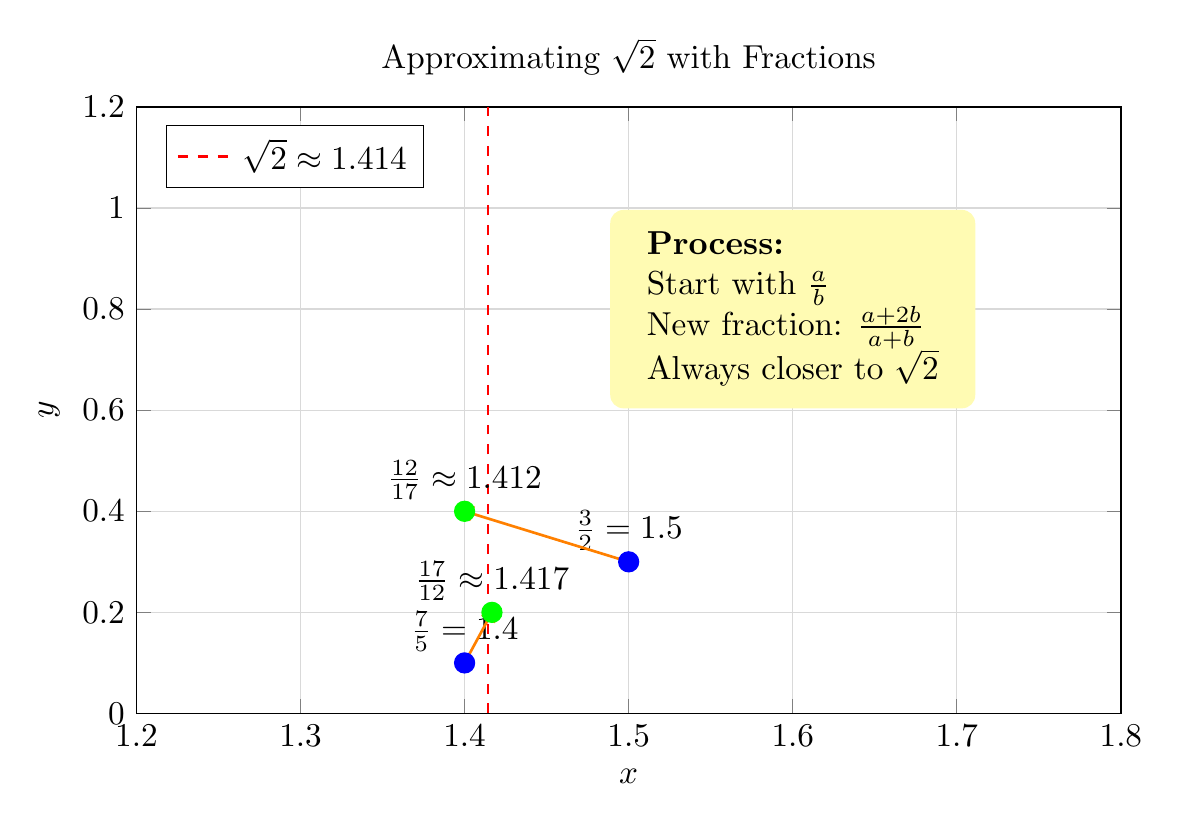
\begin{tikzpicture}[scale=1.2]
\begin{axis}[
    width=12cm,
    height=8cm,
    xlabel={$x$},
    ylabel={$y$},
    title={Approximating $\sqrt{2}$ with Fractions},
    xmin=1.2, xmax=1.8,
    ymin=0, ymax=1.2,
    grid=major,
    grid style={gray!30},
    xtick={1.2,1.3,1.4,1.5,1.6,1.7,1.8},
    ytick={0,0.2,0.4,0.6,0.8,1.0,1.2},
    legend pos=north west
]

% Plot sqrt(2) as a vertical line
\addplot[red, thick, dashed] coordinates {(1.414213562,0) (1.414213562,1.2)};
\addlegendentry{$\sqrt{2} \approx 1.414$}

% Plot some example fractions
\addplot[blue, mark=*, mark size=3pt] coordinates {(1.4,0.1)};
\node[above] at (axis cs:1.4,0.1) {$\frac{7}{5} = 1.4$};

\addplot[green, mark=*, mark size=3pt] coordinates {(1.416667,0.2)};
\node[above] at (axis cs:1.416667,0.2) {$\frac{17}{12} \approx 1.417$};

\addplot[blue, mark=*, mark size=3pt] coordinates {(1.5,0.3)};
\node[above] at (axis cs:1.5,0.3) {$\frac{3}{2} = 1.5$};

\addplot[green, mark=*, mark size=3pt] coordinates {(1.4,0.4)};
\node[above] at (axis cs:1.4,0.4) {$\frac{12}{17} \approx 1.412$};

% Add arrows showing the process
\draw[->, thick, orange] (axis cs:1.4,0.1) -- (axis cs:1.416667,0.2);
\draw[->, thick, orange] (axis cs:1.5,0.3) -- (axis cs:1.4,0.4);

% Add text explaining the process
\node[fill=yellow!30, rounded corners, inner sep=5pt] at (axis cs:1.6,0.8) {
    \begin{tabular}{l}
    \textbf{Process:} \\
    Start with $\frac{a}{b}$ \\
    New fraction: $\frac{a+2b}{a+b}$ \\
    Always closer to $\sqrt{2}$
    \end{tabular}
};

\end{axis}
\end{tikzpicture}
\end{center}

This visualization shows how the process of generating new fractions $\frac{a+2b}{a+b}$ from $\frac{a}{b}$ always produces a better approximation to $\sqrt{2}$. The red dashed line represents $\sqrt{2}$, and the arrows show the improvement in approximation.\qed


\begin{problembox}[1.14: Irrationality of $\sqrt{n - 1} + \sqrt{n + 1}$]
\begin{problemstatement}
Prove that $\sqrt{n - 1} + \sqrt{n + 1}$ is irrational for every integer $n \geq 1$.
\end{problemstatement}
\end{problembox}

\noindent\textbf{Strategy:} Use proof by contradiction. Assume the sum is rational, then square both sides to eliminate the square roots. This leads to $\sqrt{n^2 - 1}$ being rational, which is false since $n^2 - 1$ is not a perfect square for $n \geq 2$.

\bigskip\noindent\textbf{Solution:}
Assume $\sqrt{n - 1} + \sqrt{n + 1} = \frac{p}{q}$, where $p, q$ are integers, $q \neq 0$, $\gcd(p, q) = 1$.

Square both sides:
\[
(n - 1) + 2\sqrt{(n - 1)(n + 1)} + (n + 1) = \frac{p^2}{q^2} \implies 2n + 2\sqrt{n^2 - 1} = \frac{p^2}{q^2}.
\]
Thus:
\[
\sqrt{n^2 - 1} = \frac{p^2 - 2n q^2}{2 q^2}.
\]
Suppose $\sqrt{n^2 - 1}$ is rational, say $\frac{a}{b}$, $\gcd(a, b) = 1$. Then:
\[
n^2 - 1 = \frac{a^2}{b^2} \implies a^2 = (n^2 - 1)b^2.
\]
For $n = 1$, $\sqrt{0} + \sqrt{2} = \sqrt{2}$, irrational. For $n \geq 2$, $n^2 - 1 = (n - 1)(n + 1)$ is not a perfect square (since $(n - 1)^2 < n^2 - 1 < n^2$). If $a^2 = (n^2 - 1)b^2$, $n^2 - 1$ must be a perfect square, a contradiction for $n \geq 2$. Thus, $\sqrt{n^2 - 1}$ is irrational, so $\sqrt{n - 1} + \sqrt{n + 1}$ is irrational.\qed


\begin{problembox}[1.15: Approximation by Rational Numbers]
\begin{problemstatement}
Given a real $x$ and an integer $N > 1$, prove that there exist integers $h$ and $k$ with $0 < k \leq N$ such that $|kx - h| < 1/N$. Hint. Consider the $N+1$ numbers $tx-[tx]$ for $t=0,1,2,\dots,N$ and show that some pair differs by at most $1/N$.
\end{problemstatement}
\end{problembox}

\noindent\textbf{Strategy:} Use the pigeonhole principle. Consider the fractional parts of $0, x, 2x, \ldots, Nx$, divide $[0,1)$ into $N$ equal subintervals, and apply the pigeonhole principle to find two numbers in the same subinterval.

\bigskip\noindent\textbf{Solution:}
We will use the pigeonhole principle to prove this result.

Consider the $N + 1$ numbers: $0, x, 2x, 3x, \ldots, Nx$.

Let's look at the fractional parts of these numbers. The fractional part of a number $y$ is $y - \lfloor y \rfloor$, where $\lfloor y \rfloor$ is the greatest integer less than or equal to $y$.

The fractional parts of $0, x, 2x, \ldots, Nx$ all lie in the interval $[0, 1)$.

Divide the interval $[0, 1)$ into $N$ equal subintervals:
\begin{align*}
[0, 1/N), [1/N, 2/N), \ldots, [(N-1)/N, 1)
\end{align*}

By the pigeonhole principle, since we have $N + 1$ numbers and only $N$ subintervals, at least two of these numbers must fall into the same subinterval.

Let's say $ix$ and $jx$ (where $0 \leq i < j \leq N$) have fractional parts in the same subinterval. Then:
\begin{align*}
|(jx - \lfloor jx \rfloor) - (ix - \lfloor ix \rfloor)| &< \frac{1}{N} \\
|(j - i)x - (\lfloor jx \rfloor - \lfloor ix \rfloor)| &< \frac{1}{N}
\end{align*}

Let $k = j - i$ and $h = \lfloor jx \rfloor - \lfloor ix \rfloor$. Then:
\begin{align*}
|kx - h| &< \frac{1}{N}
\end{align*}

Since $0 < i < j \leq N$, we have $0 < k \leq N$, and $h$ is an integer.

Therefore, we have found integers $h$ and $k$ with $0 < k \leq N$ such that $|kx - h| < 1/N$.

\textbf{Example:}
If $x = \pi$ and $N = 5$, we might find that $3\pi \approx 9.4248$ and $5\pi \approx 15.7080$ have fractional parts in the same subinterval, giving us $|2\pi - 6| < 1/5$.\qed


\begin{problembox}[1.16: Infinitely Many Rational Approximations]
\begin{problemstatement}
If $x$ is irrational, prove that there are infinitely many rational numbers $h/k$ with $k > 0$ such that $|x - h/k| < 1/k^2$.
\end{problemstatement}
\end{problembox}

\noindent\textbf{Strategy:} We will use the result from Problem 1.15 (Dirichlet's Approximation Theorem) to construct rational approximations, then use proof by contradiction to show that there must be infinitely many distinct such approximations.

\bigskip\noindent\textbf{Solution:}
We will construct an infinite sequence of distinct rational numbers satisfying the condition.

From Problem 1.15 (Dirichlet's Approximation Theorem), for any integer $N > 1$, there exist integers $h$ and $k$ with $0 < k \leq N$ such that $|kx - h| < 1/N$.
Dividing by $k$, we get:
\[
\left|x - \frac{h}{k}\right| < \frac{1}{Nk}
\]
Since $k \leq N$, we have $\frac{1}{N} \leq \frac{1}{k}$, which implies $\frac{1}{Nk} \leq \frac{1}{k^2}$.
Thus, for any integer $N>1$, we can find a rational number $h/k$ such that:
\[
\left|x - \frac{h}{k}\right| < \frac{1}{k^2}
\]
Now we must show that this process can generate infinitely many distinct fractions.
Assume, for the sake of contradiction, that there are only a finite number of such rational approximations, say $$\{h_1/k_1, h_2/k_2, \ldots, h_m/k_m\}$$.
Since $x$ is irrational, for any rational number $h_i/k_i$, the distance $|x - h_i/k_i|$ is non-zero. Let $\epsilon$ be the smallest of these non-zero distances:
\[
\epsilon = \min_{i=1,\dots,m} \left|x - \frac{h_i}{k_i}\right| > 0.
\]
Now, choose an integer $N$ large enough such that $1/N < \epsilon$.
By the result from Problem 1.15, there exist integers $h'$ and $k'$ with $0 < k' \leq N$ such that:
\[
|k'x - h'| < \frac{1}{N}
\]
This implies $|x - h'/k'| < \frac{1}{Nk'} \leq \frac{1}{N}$.
So we have found a new rational approximation $h'/k'$ such that:
\[
\left|x - \frac{h'}{k'}\right| < \frac{1}{N} < \epsilon
\]
Since the approximation error of $h'/k'$ is smaller than $\epsilon$, $h'/k'$ cannot be one of the fractions in our finite list $\{h_1/k_1, \ldots, h_m/k_m\}$. This contradicts our assumption that we had a complete list of all such approximations.
Therefore, there must be infinitely many such rational numbers.\qed


\begin{problembox}[1.17: Factorial Representation of Rationals (Precise Form)]
\begin{problemstatement}
Let $x$ be a positive rational number of the form
\[
x = \sum_{k=1}^n \frac{a_k}{k!},
\]
where each $a_k$ is a nonnegative integer with $a_k \leq k - 1$ for $k \geq 2$ and $a_n > 0$. Let $[x]$ denote the greatest integer less than or equal to $x$. Prove that $a_1 = [x]$, that
\[
a_k = [k!x] - k[(k - 1)!x] \quad \text{for } k = 2, \dots, n,
\]
and that $n$ is the smallest integer such that $n!x$ is an integer. Conversely, show that every positive rational number $x$ can be expressed in this form in one and only one way.
\end{problemstatement}
\end{problembox}

\noindent\textbf{Strategy:} For the forward direction, use the properties of the factorial series to show that the fractional part is less than 1, then use the floor function properties. For the converse, use proof by contradiction to show uniqueness by assuming two different representations and finding a contradiction.

\bigskip\noindent\textbf{Solution:}
Let $x = \sum_{k=1}^n \frac{a_k}{k!}$ with the given conditions on $a_k$.

\textbf{1. Proof that $a_1 = [x]$:}
The sum can be written as $x = a_1 + \sum_{k=2}^n \frac{a_k}{k!}$. We must show the summation part is a positive fraction less than 1. Since $a_n > 0$, the sum is positive. We can bound the sum using the property $a_k \leq k-1$:
\[
\sum_{k=2}^n \frac{a_k}{k!} \leq \sum_{k=2}^n \frac{k-1}{k!} < \sum_{k=2}^{\infty} \frac{k-1}{k!}
\]
The infinite sum is a known identity: $\sum_{k=2}^{\infty} \frac{k-1}{k!} = \sum_{k=2}^{\infty} \left(\frac{1}{(k-1)!} - \frac{1}{k!}\right)$. This is a telescoping series whose sum is the first term, $1/(2-1)! = 1$.
Thus, $0 < \sum_{k=2}^n \frac{a_k}{k!} < 1$. This means $a_1 < x < a_1 + 1$, so by definition, $a_1 = [x]$.

\textbf{2. Formula for $a_k$:}
Define $x_1 = x - a_1 = \sum_{k=2}^n \frac{a_k}{k!}$. Then $k!x_1$ is an integer for $k \ge n$.
Consider the expression $k!x - k((k-1)!x) = k!(a_1+x_1) - k((k-1)!(a_1+x_1)) = ka_1k!/k! ...$ this gets complicated.
Let's use the given formula. Let $x_k = k!x - \sum_{j=1}^{k} a_j \frac{k!}{j!} = \sum_{j=k+1}^{n} a_j \frac{k!}{j!} = \frac{a_{k+1}}{k+1} + \frac{a_{k+2}}{(k+1)(k+2)} + \dots$.
From part (1), we know $0 \le x_k < 1$. So $[k!x] = \sum_{j=1}^{k} a_j \frac{k!}{j!}$.
Let's test the formula: $a_k = [k!x] - k[(k - 1)!x]$.
We have $[k!x] = k! \sum_{j=1}^k \frac{a_j}{j!}$ and $[(k-1)!x] = (k-1)! \sum_{j=1}^{k-1} \frac{a_j}{j!}$.
So, $[k!x] - k[(k-1)!x] = \sum_{j=1}^k a_j \frac{k!}{j!} - k \sum_{j=1}^{k-1} a_j \frac{(k-1)!}{j!} = \left(a_k + k\sum_{j=1}^{k-1} a_j \frac{(k-1)!}{j!}\right) - k\sum_{j=1}^{k-1} a_j \frac{(k-1)!}{j!} = a_k$.
This proves the formula for $a_k$.

\textbf{3. Minimality of $n$:}
Multiplying $x$ by $n!$ gives $n!x = \sum_{k=1}^n a_k \frac{n!}{k!}$. Since $k \le n$, each term $\frac{n!}{k!}$ is an integer, so $n!x$ is an integer.
For any $m < n$, when we compute $m!x$, the term corresponding to $k=n$ is $m! \frac{a_n}{n!} = \frac{a_n}{n(n-1)\dots(m+1)}$. Since $0 < a_n \le n-1$, this term is a non-integer fraction. Because all other terms for $k>m$ are also fractions and terms for $k\le m$ are integers, $m!x$ cannot be an integer. Thus, $n$ is the smallest such integer.

\textbf{4. Converse (Uniqueness):}
Suppose a positive rational number $x$ has two different representations:
\begin{align*}
x &= \sum_{k=1}^n \frac{a_k}{k!}\\
&= \sum_{k=1}^m \frac{b_k}{k!}
\end{align*}
with the conditions $0 \le a_k \le k-1$ for $k \ge 2$, $a_n > 0$, and similarly for $b_k$.
From part (3), $n$ is the smallest integer such that $n!x$ is an integer, and $m$ is the smallest integer such that $m!x$ is an integer. This implies $n=m$.

Let $j$ be the largest index for which the coefficients differ, so $a_j \neq b_j$. Assume, without loss of generality, that $a_j > b_j$.
Since $a_k = b_k$ for $k > j$, we can subtract the sums:
\begin{align*}
\sum_{k=1}^j \frac{a_k}{k!} = \sum_{k=1}^j \frac{b_k}{k!}
\end{align*}
Rearranging the terms, we get:
\begin{align*}
\frac{a_j - b_j}{j!} = \sum_{k=1}^{j-1} \frac{b_k - a_k}{k!}
\end{align*}
Multiply both sides by $(j-1)!$:
\[ \frac{a_j - b_j}{j} = \sum_{k=1}^{j-1} (b_k - a_k) \frac{(j-1)!}{k!} \]
The right-hand side is an integer, because for each $k \in \{1, \dots, j-1\}$, $k!$ divides $(j-1)!$.
Let's analyze the left-hand side. Since $a_j$ and $b_j$ are integers and $a_j > b_j$, we have $a_j - b_j \geq 1$.
From the conditions on the coefficients, $a_j \leq j-1$ (for $j \ge 2$) and $b_j \geq 0$.
Therefore, $1 \leq a_j - b_j \leq j-1$.
This implies that for $j \ge 2$, the left-hand side $\frac{a_j - b_j}{j}$ is a non-integer fraction, since the numerator is an integer between $1$ and $j-1$, and the denominator is $j$.
This creates a contradiction: the left-hand side cannot be an integer, while the right-hand side must be an integer.
For the case $j=1$, the equation becomes $a_1 - b_1 = 0$, which contradicts $a_1 \neq b_1$.
Thus, our assumption that there is a largest index $j$ where $a_j \neq b_j$ must be false. All coefficients must be identical. The representation is unique.

\textit{5. Uniqueness:} Suppose $x$ has two different representations, $\sum \frac{a_k}{k!} = \sum \frac{b_k}{k!}$. Let $j$ be the largest index where $a_j \neq b_j$. Assume $a_j > b_j$. Then $\frac{a_j - b_j}{j!} = \sum_{k=1}^{j-1} \frac{b_k - a_k}{k!}$. The left side is $\ge 1/j!$. The right side is bounded above by $\sum_{k=1}^{j-1} \frac{k-1}{k!} < 1/j!$, a contradiction. Thus, all coefficients must be the same.\qed
\section{Upper Bounds}

\subsection*{Definitions and Theorems for Upper Bounds}

\begin{definition}[Upper Bound]
A real number $M$ is an upper bound for a set $S \subseteq \mathbb{R}$ if $x \leq M$ for all $x \in S$.
\end{definition}

\begin{definition}[Lower Bound]
A real number $m$ is a lower bound for a set $S \subseteq \mathbb{R}$ if $x \geq m$ for all $x \in S$.
\end{definition}

\begin{definition}[Supremum]
The supremum (least upper bound) of a set $S \subseteq \mathbb{R}$, denoted $\sup S$, is the smallest real number that is an upper bound for $S$.
\end{definition}

\begin{definition}[Infimum]
The infimum (greatest lower bound) of a set $S \subseteq \mathbb{R}$, denoted $\inf S$, is the largest real number that is a lower bound for $S$.
\end{definition}

\begin{theorem}[Completeness Axiom]
Every nonempty set of real numbers that is bounded above has a supremum.
\end{theorem}

\begin{theorem}[Uniqueness of Supremum and Infimum]
If a set has a supremum (infimum), it is unique.
\end{theorem}

\begin{theorem}[Archimedean Property]
For any positive real numbers $a$ and $b$, there exists a positive integer $n$ such that $na > b$.
\end{theorem}

\begin{theorem}[Comparison Property for Suprema]
Let $S$ and $T$ be nonempty subsets of $\mathbb{R}$ such that $s \leq t$ for all $s \in S$ and $t \in T$. If $T$ has a supremum, then $S$ has a supremum and $\sup S \leq \sup T$.
\end{theorem}




\begin{problembox}[1.18: Uniqueness of Supremum and Infimum]
\begin{problemstatement}
Show that the $\sup$ and $\inf$ of a set are uniquely determined whenever they exist.
\end{problemstatement}
\end{problembox}

\noindent\textbf{Strategy:} We will prove the uniqueness of supremum by contradiction, assuming there are two different suprema and showing this leads to a contradiction. The same approach applies to infimum.

\bigskip\noindent\textbf{Solution:}
We will prove that if a set has a supremum, it is unique. The proof for infimum is similar.

\textbf{Proof by contradiction:}
Suppose a set $S$ has two different suprema, say $s_1$ and $s_2$, with $s_1 < s_2$.

Since $s_1$ is a supremum of $S$:
1. $s_1$ is an upper bound of $S$ (every element of $S$ is $\leq s_1$)
2. $s_1$ is the least upper bound (no number less than $s_1$ is an upper bound)

Since $s_2$ is also a supremum of $S$:
1. $s_2$ is an upper bound of $S$ (every element of $S$ is $\leq s_2$)
2. $s_2$ is the least upper bound (no number less than $s_2$ is an upper bound)

But since $s_1 < s_2$, the number $s_1$ is less than $s_2$ and is also an upper bound of $S$. This contradicts the fact that $s_2$ is the least upper bound.

Therefore, our assumption that there are two different suprema is false, and the supremum must be unique.

\textbf{Alternative proof:}
Let $s_1$ and $s_2$ both be suprema of $S$. Then:
- $s_1$ is an upper bound, so $s_2 \leq s_1$ (since $s_2$ is the least upper bound)
- $s_2$ is an upper bound, so $s_1 \leq s_2$ (since $s_1$ is the least upper bound)

Therefore, $s_1 = s_2$.

\textbf{For infimum:}
The same argument applies to infimum. If a set has two infima $i_1$ and $i_2$, then:
- $i_1$ is a lower bound, so $i_1 \leq i_2$ (since $i_1$ is the greatest lower bound)
- $i_2$ is a lower bound, so $i_2 \leq i_1$ (since $i_2$ is the greatest lower bound)

Therefore, $i_1 = i_2$.\qed


\begin{problembox}[1.19: Finding Supremum and Infimum]
\begin{problemstatement}
Find the $\sup$ and $\inf$ of each of the following sets:
\begin{enumerate}[label=(\alph*)]
\item All numbers of the form $2^{-p} + 3^{-q} + 5^{-r}$ for positive integers $p, q, r$.
\item $S = \{x : 3x^2 - 10x + 3 < 0\}$.
\item $S = \{x : (x - a)(x - b)(x - c)(x - d) < 0\}$ where $a < b < c < d$.
\end{enumerate}
\end{problemstatement}
\end{problembox}

\noindent\textbf{Strategy:} For (a), analyze the range of each exponential term and find the maximum and minimum values. For (b), solve the quadratic inequality to find the interval. For (c), use the sign changes of the polynomial at its roots to determine the intervals where the product is negative.

\bigskip\noindent\textbf{Solution:}

\textbf{1. Numbers of the form $2^{-p} + 3^{-q} + 5^{-r}$:}

Let's analyze the range of each term:
- $2^{-p}$ ranges from $\frac{1}{2}$ (when $p = 1$) to $0$ (as $p \to \infty$)
- $3^{-q}$ ranges from $\frac{1}{3}$ (when $q = 1$) to $0$ (as $q \to \infty$)
- $5^{-r}$ ranges from $\frac{1}{5}$ (when $r = 1$) to $0$ (as $r \to \infty$)

Therefore:
- The maximum value occurs when $p = q = r = 1$: $\frac{1}{2} + \frac{1}{3} + \frac{1}{5} = \frac{15 + 10 + 6}{30} = \frac{31}{30}$
- The minimum value occurs as $p, q, r \to \infty$: $0 + 0 + 0 = 0$

So $\sup = \textbf{$\frac{31}{30}$}$ and $\inf = \textbf{$0$}$.

\textbf{2. Set $S = \{x : 3x^2 - 10x + 3 < 0\}$:}

First, let's find the roots of $3x^2 - 10x + 3 = 0$:
\begin{align*}
x &= \frac{10 \pm \sqrt{100 - 36}}{6} \\
&= \frac{10 \pm \sqrt{64}}{6} \\
&= \frac{10 \pm 8}{6} \\
&= \frac{18}{6} = 3 \quad \text{or} \quad \frac{2}{6} = \frac{1}{3}
\end{align*}

Since the coefficient of $x^2$ is positive, the parabola opens upward. The inequality $3x^2 - 10x + 3 < 0$ holds between the roots.

Therefore, $S = (\frac{1}{3}, 3)$, so $\sup = \textbf{$3$}$ and $\inf = \textbf{$\frac{1}{3}$}$.

\textbf{Visualization for part (b):}
\begin{center}
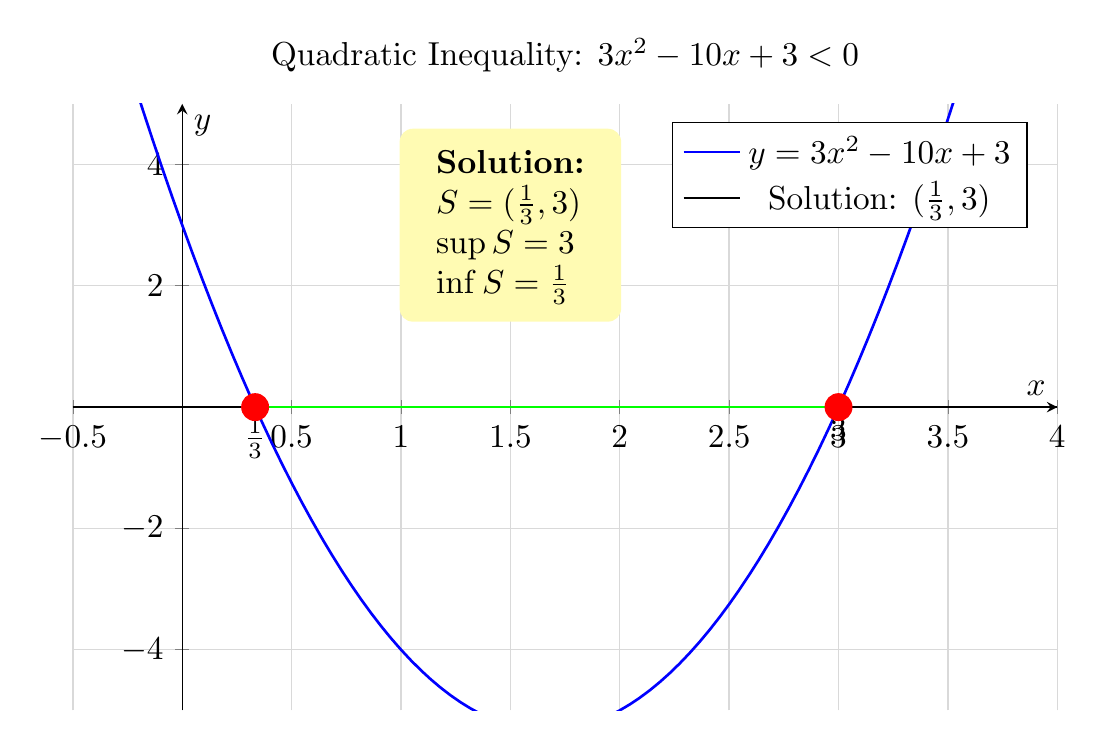
\begin{tikzpicture}[scale=1.2]
\begin{axis}[
    width=12cm,
    height=8cm,
    xlabel={$x$},
    ylabel={$y$},
    title={Quadratic Inequality: $3x^2 - 10x + 3 < 0$},
    xmin=-0.5, xmax=4,
    ymin=-5, ymax=5,
    grid=major,
    grid style={gray!30},
    axis lines=middle,
    legend pos=north east
]

% Plot the quadratic function
\addplot[blue, thick, samples=100, domain=-0.5:4] {3*x^2 - 10*x + 3};
\addlegendentry{$y = 3x^2 - 10x + 3$}

% Plot the x-axis
\addplot[black, thick] coordinates {(-0.5,0) (4,0)};

% Mark the roots
\addplot[red, mark=*, mark size=4pt] coordinates {(0.333,0) (3,0)};
\node[below] at (axis cs:0.333,0) {$\frac{1}{3}$};
\node[below] at (axis cs:3,0) {$3$};

% Highlight the solution interval
\addplot[green, fill=green!20, fill opacity=0.3] coordinates {(0.333,0) (3,0)};
\addplot[green, thick] coordinates {(0.333,0) (3,0)};
\addlegendentry{Solution: $(\frac{1}{3}, 3)$}

% Add text explaining the solution
\node[fill=yellow!30, rounded corners, inner sep=5pt] at (axis cs:1.5,3) {
    \begin{tabular}{l}
    \textbf{Solution:} \\
    $S = (\frac{1}{3}, 3)$ \\
    $\sup S = 3$ \\
    $\inf S = \frac{1}{3}$
    \end{tabular}
};

\end{axis}
\end{tikzpicture}
\end{center}

This visualization shows the quadratic function $y = 3x^2 - 10x + 3$ and highlights the interval where the inequality $3x^2 - 10x + 3 < 0$ holds, which is between the roots $\frac{1}{3}$ and $3$.

\textbf{3. Set $S = \{x : (x - a)(x - b)(x - c)(x - d) < 0\}$ where $a < b < c < d$:}

The expression $(x - a)(x - b)(x - c)(x - d)$ changes sign at each root $a, b, c, d$.

Starting from $-\infty$:
- For $x < a$: all factors are negative, so the product is positive
- For $a < x < b$: one factor is positive, three negative, so product is negative
- For $b < x < c$: two factors positive, two negative, so product is positive
- For $c < x < d$: three factors positive, one negative, so product is negative
- For $x > d$: all factors are positive, so product is positive

Therefore, $S = (a, b) \cup (c, d)$.

So $\sup = \textbf{$d$}$ and $\inf = \textbf{$a$}$.

\textbf{Visualization for part (c):}
\begin{center}
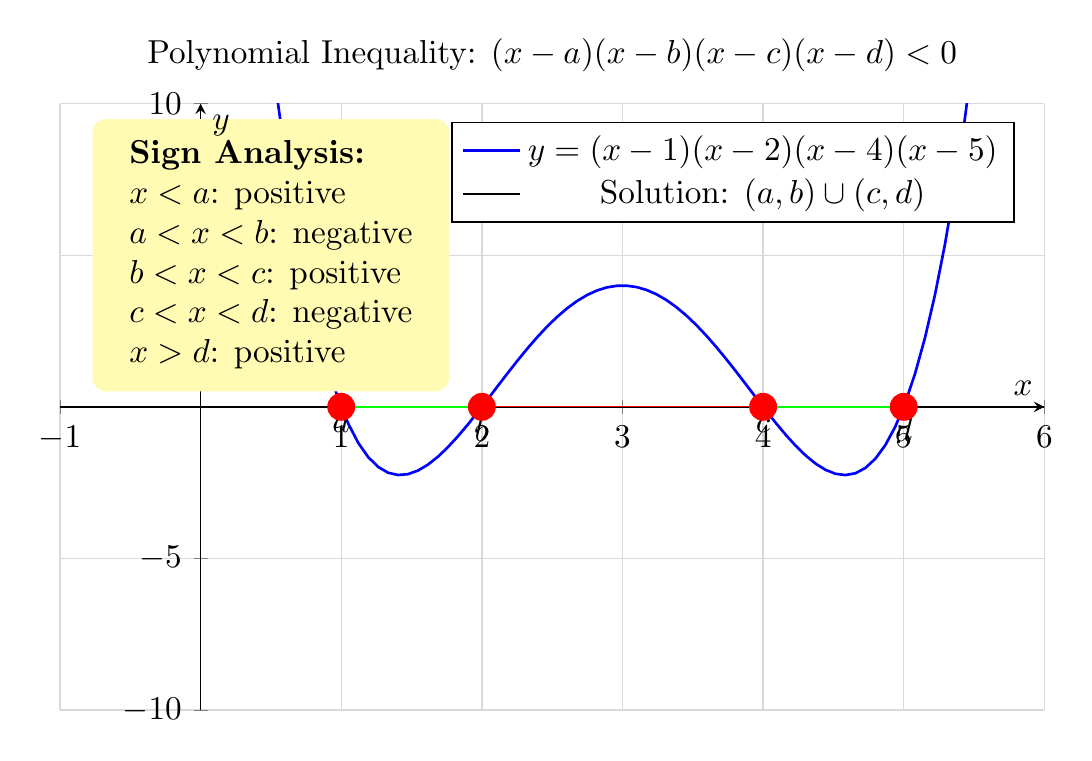
\begin{tikzpicture}[scale=1.2]
\begin{axis}[
    width=12cm,
    height=8cm,
    xlabel={$x$},
    ylabel={$y$},
    title={Polynomial Inequality: $(x-a)(x-b)(x-c)(x-d) < 0$},
    xmin=-1, xmax=6,
    ymin=-10, ymax=10,
    grid=major,
    grid style={gray!30},
    axis lines=middle,
    legend pos=north east
]

% Example with a=1, b=2, c=4, d=5
\addplot[blue, thick, samples=100, domain=-1:6] {(x-1)*(x-2)*(x-4)*(x-5)};
\addlegendentry{$y = (x-1)(x-2)(x-4)(x-5)$}

% Plot the x-axis
\addplot[black, thick] coordinates {(-1,0) (6,0)};

% Mark the roots
\addplot[red, mark=*, mark size=4pt] coordinates {(1,0) (2,0) (4,0) (5,0)};
\node[below] at (axis cs:1,0) {$a$};
\node[below] at (axis cs:2,0) {$b$};
\node[below] at (axis cs:4,0) {$c$};
\node[below] at (axis cs:5,0) {$d$};

% Highlight the solution intervals
\addplot[green, fill=green!20, fill opacity=0.3] coordinates {(1,0) (2,0)};
\addplot[green, thick] coordinates {(1,0) (2,0)};
\addplot[green, fill=green!20, fill opacity=0.3] coordinates {(4,0) (5,0)};
\addplot[green, thick] coordinates {(4,0) (5,0)};
\addlegendentry{Solution: $(a,b) \cup (c,d)$}

% Add text explaining the sign changes
\node[fill=yellow!30, rounded corners, inner sep=5pt] at (axis cs:0.5,5) {
    \begin{tabular}{l}
    \textbf{Sign Analysis:} \\
    $x < a$: positive \\
    $a < x < b$: negative \\
    $b < x < c$: positive \\
    $c < x < d$: negative \\
    $x > d$: positive
    \end{tabular}
};

\end{axis}
\end{tikzpicture}
\end{center}

This visualization shows the fourth-degree polynomial $(x-a)(x-b)(x-c)(x-d)$ and highlights the intervals where the inequality $(x-a)(x-b)(x-c)(x-d) < 0$ holds. The polynomial changes sign at each root, creating alternating positive and negative intervals.\qed


\begin{problembox}[1.20: Comparison Property for Suprema]
\begin{problemstatement}
Let \( S \) and \( T \) be nonempty subsets of \( \mathbb{R} \) such that \( s \leq t \) for all \( s \in S \) and \( t \in T \). Suppose \( T \) has a supremum. Then \( S \) has a supremum and
\[
\sup S \leq \sup T.
\]
\end{problemstatement}
\end{problembox}

\noindent\textbf{Strategy:} We will first show that $S$ has a supremum by using the completeness axiom, then prove that $\sup S \leq \sup T$ by showing that $\sup S$ is a lower bound for $T$ and using the definition of supremum.

\bigskip\noindent\textbf{Solution:}
Let $S$ and $T$ be nonempty subsets of $\mathbb{R}$ with the property that for every $s \in S$ and $t \in T$, we have $s \leq t$.

1.  \textbf{Existence of $\sup S$}:
Since $T$ is nonempty, we can pick an arbitrary element $t_0 \in T$. By the given property, for every $s \in S$, we have $s \leq t_0$. This shows that $S$ is bounded above (by any element of $T$). Since $S$ is also nonempty and bounded above, the completeness axiom of $\mathbb{R}$ guarantees that $\sup S$ exists. Let's call it $\alpha = \sup S$.

2.  \textbf{Proof that $\sup S \leq \sup T$}:
Let $\alpha = \sup S$ and $\beta = \sup T$.
From step 1, we know that any element $t \in T$ is an upper bound for the set $S$.
Since $\alpha$ is the *least* upper bound of $S$, it must be less than or equal to any other upper bound of $S$. Therefore, for any $t \in T$, we must have:
\[
\alpha \leq t
\]
This inequality shows that $\alpha$ is a lower bound for the set $T$.
Now, by definition, $\beta = \sup T$ is the least upper bound of $T$. As an upper bound for $T$, $\beta$ must be greater than or equal to every element of $T$. More importantly, it must be greater than or equal to any *lower bound* of $T$.
Since we have established that $\alpha$ is a lower bound for $T$, it must follow that:
\[
\alpha \leq \beta
\]
Substituting the definitions of $\alpha$ and $\beta$, we get:
\[
\sup S \leq \sup T
\]
This completes the proof.\qed


\begin{problembox}[1.21: Product of Suprema]
\begin{problemstatement}
Let \( A \) and \( B \) be two sets of positive real numbers, each bounded above. Let \( a = \sup A \), \( b = \sup B \). Define
\[
C = \{ xy : x \in A,\, y \in B \}.
\]
Prove that
\[
\sup C = ab.
\]
\end{problemstatement}
\end{problembox}

\noindent\textbf{Strategy:} We will show that $ab$ is an upper bound for $C$, then prove it is the least upper bound by using the definition of supremum and constructing elements of $C$ that are arbitrarily close to $ab$.

\bigskip\noindent\textbf{Solution:}

Since \( A \) and \( B \) are sets of positive real numbers bounded above, their suprema \( a = \sup A \) and \( b = \sup B \) exist and are finite.

We are to prove that:
\[
\sup C = ab.
\]

\textbf{Step 1: Show that \( ab \) is an upper bound for \( C \).}

Let \( x \in A \), \( y \in B \). Since \( x \leq a \) and \( y \leq b \), we have:
\[
xy \leq ab.
\]
Therefore, every element \( c \in C \) satisfies \( c \leq ab \), so \( ab \) is an upper bound for \( C \).

\textbf{Step 2: Show that \( ab \) is the least upper bound.}

Let \( \varepsilon > 0 \). Since \( a = \sup A \), there exists \( x_\varepsilon \in A \) such that:
\[
x_\varepsilon > a - \frac{\varepsilon}{2b}.
\]
Similarly, since \( b = \sup B \), there exists \( y_\varepsilon \in B \) such that:
\[
y_\varepsilon > b - \frac{\varepsilon}{2a}.
\]

Now consider:
\[
x_\varepsilon y_\varepsilon > \left(a - \frac{\varepsilon}{2b}\right)\left(b - \frac{\varepsilon}{2a}\right) = ab - \frac{\varepsilon}{2} - \frac{\varepsilon}{2} + \frac{\varepsilon^2}{4ab}.
\]
Since \( \frac{\varepsilon^2}{4ab} > 0 \), we have:
\[
x_\varepsilon y_\varepsilon > ab - \varepsilon.
\]
Therefore, for every \( \varepsilon > 0 \), there exists \( c \in C \) such that \( c > ab - \varepsilon \). Hence, \( ab \) is the least upper bound of \( C \).

\[
\boxed{\sup C = ab}
\]\qed


\begin{problembox}[1.22: Representation of Rationals in Base \( k \)]
\begin{problemstatement}
Given \( x \geq 0 \) and an integer \( k \geq 2 \), let \( a_0 \) denote the largest integer \( \leq x \), and, assuming that \( a_0, a_1, \dots, a_{n-1} \) have been defined, let \( a_n \) denote the largest integer such that
\[
a_0 + \frac{a_1}{k} + \frac{a_2}{k^2} + \cdots + \frac{a_n}{k^n} \leq x.
\]

\begin{enumerate}
\item[(a)] Prove that \( 0 \leq a_i \leq k - 1 \) for each \( i = 1, 2, \dots \).
\item[(b)] Let \( r_n = a_0 + a_1 k^{-1} + a_2 k^{-2} + \cdots + a_n k^{-n} \) and show that \( x = \sup \{ r_n \} \), the supremum of the set of rational numbers \( r_1, r_2, \dots \).
\end{enumerate}
\end{problemstatement}
\end{problembox}

\noindent\textbf{Strategy:} For (a), use the definition of $a_n$ as the largest integer satisfying the condition and show that choosing $a_n + 1$ would violate it. For (b), use the Archimedean property and proof by contradiction to show that the supremum equals $x$.

\bigskip\noindent\textbf{Solution:}
Let \( r_n = \sum_{i=0}^n \frac{a_i}{k^i} \). By definition, \( a_n \) is the largest integer such that \( r_n \leq x \).

\textbf{(a) Show \( 0 \leq a_i \leq k - 1 \):}
Since \( a_n \) is the largest integer satisfying the condition, choosing \( a_n + 1 \) would violate it:
\[
r_{n-1} + \frac{a_n + 1}{k^n} > x
\]
From the definition of \(a_{n-1}\), we know it was the largest integer such that \( r_{n-1} \le x \). This implies $x - r_{n-1} < \frac{1}{k^{n-1}}$.
Now, from the definition of $a_n$, we have $r_{n-1} + \frac{a_n}{k^n} \leq x$, which implies $a_n \leq k^n(x - r_{n-1})$.
Combining these facts:
\[
a_n \leq k^n(x - r_{n-1}) < k^n\left(\frac{1}{k^{n-1}}\right) = k.
\]
Since $a_n$ is an integer and $a_n < k$, we must have $a_n \leq k-1$. Also, $a_n$ must be non-negative, otherwise we could choose $a_n=0$ to get a larger (or equal) sum $r_n$ that is still less than or equal to $x$, contradicting the "largest integer" definition if the original $a_n$ were negative. Thus, $0 \leq a_n \leq k-1$.

\textbf{(b) Show that \( x = \sup \{ r_n \} \):}
The sequence $\{r_n\}$ is non-decreasing by construction, since $a_n \ge 0$. It is also bounded above by $x$. Therefore, its supremum exists; let $r = \sup\{r_n\}$. We know $r \le x$.
We will prove $r=x$ by contradiction. Assume $r < x$. Let $\delta = x - r > 0$.
By the Archimedean property, we can choose an integer $N$ large enough such that $\frac{1}{k^N} < \delta$.
From the definition of $a_N$, we know $r_N = r_{N-1} + \frac{a_N}{k^N} \le x$ and $r_{N-1} + \frac{a_N+1}{k^N} > x$.
The second inequality rearranges to $x - r_N < \frac{1}{k^N}$.
Since $r = \sup\{r_n\}$, we know $r_N \leq r$.
Therefore, $x - r \leq x - r_N < \frac{1}{k^N}$.
Substituting $\delta = x-r$, we get $\delta < \frac{1}{k^N}$.
But we chose $N$ such that $\frac{1}{k^N} < \delta$. This gives $\delta < \frac{1}{k^N} < \delta$, a contradiction.
Thus, our assumption must be false, and $x = r = \sup\{r_n\}$.\qed
\section{Inequalities and Identities}

\subsection*{Additional Theorems for Inequalities and Identities}

\begin{theorem}[Binomial Theorem]
For any real numbers $a$ and $b$ and positive integer $n$:
\[
(a + b)^n = \sum_{k=0}^n \binom{n}{k} a^{n-k} b^k
\]
\end{theorem}

\begin{theorem}[Pigeonhole Principle]
If $n$ objects are placed into $m$ containers where $n > m$, then at least one container must contain more than one object.
\end{theorem}

\begin{theorem}[Dirichlet's Approximation Theorem]
For any real number $x$ and positive integer $N$, there exist integers $h$ and $k$ with $0 < k \leq N$ such that $|kx - h| < 1/N$.
\end{theorem}



\begin{problembox}[1.23: Lagrange's Identity]
\begin{problemstatement}
Prove Lagrange's identity for real numbers:
\[
\left( \sum_{k=1}^n a_k b_k \right)^2 = \left( \sum_{k=1}^n a_k^2 \right)\left( \sum_{k=1}^n b_k^2 \right) - \sum_{1 \leq k < j \leq n} (a_k b_j - a_j b_k)^2.
\]
\end{problemstatement}
\end{problembox}

\noindent\textbf{Strategy:} We will prove this identity by expanding both sides and showing they are equal. We'll expand the left-hand side as a double sum and the right-hand side by expanding the product and the squared terms, then show that all terms cancel appropriately.

\bigskip\noindent\textbf{Solution:}
We will prove Lagrange's identity by expanding both sides and showing they are equal.

Let's start by expanding the left-hand side:
\begin{align*}
\left( \sum_{k=1}^n a_k b_k \right)^2 &= \left( \sum_{k=1}^n a_k b_k \right) \left( \sum_{j=1}^n a_j b_j \right) \\
&= \sum_{k=1}^n \sum_{j=1}^n a_k b_k a_j b_j \\
&= \sum_{k=1}^n a_k^2 b_k^2 + 2 \sum_{1 \leq k < j \leq n} a_k b_k a_j b_j
\end{align*}

Now let's expand the right-hand side:
\begin{align*}
&\left( \sum_{k=1}^n a_k^2 \right)\left( \sum_{k=1}^n b_k^2 \right) - \sum_{1 \leq k < j \leq n} (a_k b_j - a_j b_k)^2 \\
&= \left( \sum_{k=1}^n a_k^2 \right)\left( \sum_{j=1}^n b_j^2 \right) - \sum_{1 \leq k < j \leq n} (a_k^2 b_j^2 - 2a_k b_j a_j b_k + a_j^2 b_k^2) \\
&= \sum_{k=1}^n \sum_{j=1}^n a_k^2 b_j^2 - \sum_{1 \leq k < j \leq n} a_k^2 b_j^2 + 2 \sum_{1 \leq k < j \leq n} a_k b_j a_j b_k - \sum_{1 \leq k < j \leq n} a_j^2 b_k^2
\end{align*}

Let's simplify this step by step. First, note that:
\begin{align*}
\sum_{k=1}^n \sum_{j=1}^n a_k^2 b_j^2 &= \sum_{k=1}^n a_k^2 b_k^2 + \sum_{1 \leq k < j \leq n} a_k^2 b_j^2 + \sum_{1 \leq k < j \leq n} a_j^2 b_k^2 \\
&= \sum_{k=1}^n a_k^2 b_k^2 + \sum_{1 \leq k < j \leq n} (a_k^2 b_j^2 + a_j^2 b_k^2)
\end{align*}

Substituting this back into our expression:
\begin{align*}
&\sum_{k=1}^n a_k^2 b_k^2 + \sum_{1 \leq k < j \leq n} (a_k^2 b_j^2 + a_j^2 b_k^2) - \sum_{1 \leq k < j \leq n} a_k^2 b_j^2 + 2 \sum_{1 \leq k < j \leq n} a_k b_j a_j b_k  \\
&- \sum_{1 \leq k < j \leq n} a_j^2 b_k^2 \\
=& \sum_{k=1}^n a_k^2 b_k^2 + 2 \sum_{1 \leq k < j \leq n} a_k b_j a_j b_k
\end{align*}

This is exactly the same as our expanded left-hand side! Therefore, Lagrange's identity is proven.

\textbf{Alternative Proof using Determinants:}
We can also prove this using the fact that the determinant of a 2×2 matrix is zero if and only if its rows are linearly dependent.

Consider the matrix:
\[
\begin{pmatrix}
a_k & b_k \\
a_j & b_j
\end{pmatrix}
\]

The determinant of this matrix is $a_k b_j - a_j b_k$. If we square this determinant and sum over all pairs $(k,j)$ with $k < j$, we get the right-hand side of Lagrange's identity.

The left-hand side represents the square of the dot product of the vectors $\mathbf{a} = (a_1, a_2, \ldots, a_n)$ and $\mathbf{b} = (b_1, b_2, \ldots, b_n)$.

The identity shows that the square of the dot product equals the product of the squared magnitudes minus the sum of squared determinants of all 2×2 submatrices formed by pairs of components.\qed


\begin{problembox}[1.24: A Holder-type Inequality]
\begin{problemstatement}
Prove that for arbitrary real numbers \( a_k, b_k, c_k \) we have
\[
\left( \sum_{k=1}^n a_k b_k c_k \right)^4 \leq
\left( \sum_{k=1}^n a_k^4 \right)
\left( \sum_{k=1}^n b_k^2 \right)^2
\left( \sum_{k=1}^n c_k^4 \right).
\]
\end{problemstatement}
\end{problembox}

\noindent\textbf{Strategy:} We will apply the Cauchy-Schwarz inequality twice. First, we'll group $(a_k c_k)$ and $b_k$, then apply Cauchy-Schwarz to the resulting term $\sum_{k=1}^n a_k^2 c_k^2$ by treating it as the dot product of sequences $\{a_k^2\}$ and $\{c_k^2\}$.

\bigskip\noindent\textbf{Solution:}
We will prove this inequality by applying the Cauchy-Schwarz inequality twice.
First, group the terms as $(a_k c_k)$ and $b_k$. Applying the Cauchy-Schwarz inequality to the sequences $\{a_k c_k\}$ and $\{b_k\}$ gives:
\[
\left( \sum_{k=1}^n (a_k c_k) b_k \right)^2 \leq \left( \sum_{k=1}^n (a_k c_k)^2 \right) \left( \sum_{k=1}^n b_k^2 \right) = \left( \sum_{k=1}^n a_k^2 c_k^2 \right) \left( \sum_{k=1}^n b_k^2 \right).
\]
Next, we apply the Cauchy-Schwarz inequality to the term $\sum_{k=1}^n a_k^2 c_k^2$, treating it as the dot product of sequences $\{a_k^2\}$ and $\{c_k^2\}$:
\[
\left( \sum_{k=1}^n a_k^2 c_k^2 \right)^2 \leq \left( \sum_{k=1}^n (a_k^2)^2 \right) \left( \sum_{k=1}^n (c_k^2)^2 \right) = \left( \sum_{k=1}^n a_k^4 \right) \left( \sum_{k=1}^n c_k^4 \right).
\]
This implies:
\[
\sum_{k=1}^n a_k^2 c_k^2 \leq \left( \sum_{k=1}^n a_k^4 \right)^{1/2} \left( \sum_{k=1}^n c_k^4 \right)^{1/2}.
\]
Now, substitute this result back into our first inequality:
\[
\left( \sum_{k=1}^n a_k b_k c_k \right)^2 \leq \left( \sum_{k=1}^n a_k^4 \right)^{1/2} \left( \sum_{k=1}^n c_k^4 \right)^{1/2} \left( \sum_{k=1}^n b_k^2 \right).
\]
Finally, squaring both sides gives the desired result:
\[
\left( \sum_{k=1}^n a_k b_k c_k \right)^4 \leq \left( \sum_{k=1}^n a_k^4 \right) \left( \sum_{k=1}^n c_k^4 \right) \left( \sum_{k=1}^n b_k^2 \right)^2.
\]\qed


\begin{problembox}[1.25: Minkowski's Inequality]
\begin{problemstatement}
Prove Minkowski's inequality:
\[
\left( \sum_{k=1}^n (a_k + b_k)^2 \right)^{1/2} \leq \left( \sum_{k=1}^n a_k^2 \right)^{1/2} + \left( \sum_{k=1}^n b_k^2 \right)^{1/2}.
\]
\end{problemstatement}
\end{problembox}

\noindent\textbf{Strategy:} We will expand the left-hand side, apply the Cauchy-Schwarz inequality to the cross term, then complete the square to obtain the desired inequality.

\bigskip\noindent\textbf{Solution:}

Let \( A = \left( \sum a_k^2 \right)^{1/2} \), \( B = \left( \sum b_k^2 \right)^{1/2} \), and expand the square:
\[
\sum (a_k + b_k)^2 = \sum a_k^2 + 2\sum a_k b_k + \sum b_k^2 = A^2 + 2\sum a_k b_k + B^2.
\]

Apply Cauchy–Schwarz:
\[
\sum a_k b_k \leq A B.
\]
Thus,
\[
\sum (a_k + b_k)^2 \leq A^2 + 2AB + B^2 = (A + B)^2.
\]
Taking square roots:
\[
\left( \sum (a_k + b_k)^2 \right)^{1/2} \leq A + B.
\]\qed


\begin{problembox}[1.26: Chebyshev's Sum Inequality]
\begin{problemstatement}
If \( a_1 \geq a_2 \geq \cdots \geq a_n \) and \( b_1 \geq b_2 \geq \cdots \geq b_n \), prove that
\[
\left( \sum_{k=1}^n a_k \right)\left( \sum_{k=1}^n b_k \right) \leq n \sum_{k=1}^n a_k b_k.
\]
\end{problemstatement}
\end{problembox}

\noindent\textbf{Strategy:} We will consider the double summation $S = \sum_{i=1}^n \sum_{j=1}^n (a_i - a_j)(b_i - b_j)$ and show that it is non-negative due to the ordering of the sequences, then expand it to obtain the desired inequality.

\bigskip\noindent\textbf{Solution:}
Consider the double summation
\[ S = \sum_{i=1}^n \sum_{j=1}^n (a_i - a_j)(b_i - b_j). \]
Since the sequences $\{a_k\}$ and $\{b_k\}$ are sorted in the same order (both non-increasing), the terms $(a_i - a_j)$ and $(b_i - b_j)$ always have the same sign. If $i>j$, then $a_i \le a_j$ and $b_i \le b_j$, so both differences are non-positive. If $i<j$, both are non-negative. Therefore, their product is always non-negative:
\[ (a_i - a_j)(b_i - b_j) \geq 0. \]
This implies that the total sum $S$ must be non-negative, $S \geq 0$.

Now, let's expand the sum:
\begin{align*}
S &= \sum_{i=1}^n \sum_{j=1}^n (a_i b_i - a_i b_j - a_j b_i + a_j b_j) \\
&= \sum_{i=1}^n \sum_{j=1}^n a_i b_i - \sum_{i=1}^n \sum_{j=1}^n a_i b_j - \sum_{i=1}^n \sum_{j=1}^n a_j b_i + \sum_{i=1}^n \sum_{j=1}^n a_j b_j
\end{align*}
We evaluate each double summation:
\begin{itemize}
\item \( \sum_{i=1}^n \sum_{j=1}^n a_i b_i = \sum_{i=1}^n \left( n \cdot a_i b_i \right) = n \sum_{i=1}^n a_i b_i \)
\item \( \sum_{i=1}^n \sum_{j=1}^n a_i b_j = \left( \sum_{i=1}^n a_i \right) \left( \sum_{j=1}^n b_j \right) \)
\item \( \sum_{i=1}^n \sum_{j=1}^n a_j b_i = \left( \sum_{j=1}^n a_j \right) \left( \sum_{i=1}^n b_i \right) \)
\item \( \sum_{i=1}^n \sum_{j=1}^n a_j b_j = \sum_{j=1}^n \left( n \cdot a_j b_j \right) = n \sum_{j=1}^n a_j b_j \)
\end{itemize}
Substituting these back into the expression for $S$:
\[
S = n \sum a_k b_k - \left(\sum a_k\right)\left(\sum b_k\right) - \left(\sum a_k\right)\left(\sum b_k\right) + n \sum a_k b_k
\]
\[
S = 2n \sum_{k=1}^n a_k b_k - 2 \left( \sum_{k=1}^n a_k \right) \left( \sum_{k=1}^n b_k \right)
\]
Since we established that $S \geq 0$:
\[
2n \sum_{k=1}^n a_k b_k - 2 \left( \sum_{k=1}^n a_k \right) \left( \sum_{k=1}^n b_k \right) \geq 0
\]
Dividing by 2 and rearranging gives the desired inequality:
\[
n \sum_{k=1}^n a_k b_k \geq \left( \sum_{k=1}^n a_k \right) \left( \sum_{k=1}^n b_k \right).
\]\qed

\section{Complex Numbers}

\begin{problembox}[1.27: Express Complex Numbers in $a + bi$ Form]
\begin{problemstatement}
Express the following complex numbers in the form \( a + bi \):

\begin{enumerate}
\item[(a)] \( (1 + i)^3 \)
\item[(b)] \( \frac{2 + 3i}{3 - 4i} \)
\item[(c)] \( i^5 + i^{16} \)
\item[(d)] \( \frac{1}{2}(1 + i)(1 + i^{-8}) \)
\end{enumerate}
\end{problemstatement}
\end{problembox}

\noindent\textbf{Strategy:} We will use the properties of complex numbers, including $i^2 = -1$, $i^4 = 1$, and the fact that powers of $i$ cycle every 4. For division, we'll rationalize the denominator by multiplying by the complex conjugate.

\bigskip\noindent\textbf{Solution:}

\begin{itemize}
\item[(a)] \( (1 + i)^3 = (1 + i)^2 (1 + i) = (2i)(1 + i) = 2i + 2i^2 = 2i - 2 = -2 + 2i \)

\item[(b)] Rationalize the denominator:
\begin{align*}
\frac{2 + 3i}{3 - 4i} \cdot \frac{3 + 4i}{3 + 4i} =& \frac{(2 + 3i)(3 + 4i)}{9 + 16} = \frac{6 + 8i + 9i + 12i^2}{25} \\
=& \frac{-6 + 17i}{25} = -\frac{6}{25} + \frac{17}{25}i
\end{align*}

\item[(c)] \( i^5 = i \), since \( i^4 = 1 \), and \( i^{16} = (i^4)^4 = 1 \), so:
\[
i^5 + i^{16} = i + 1 = 1 + i
\]

\item[(d)] \( \frac{1}{2}(1 + i)(1 + i^{-8}) \), note that \( i^{-8} = (i^4)^{-2} = 1^{-2} = 1 \), so:
\[
\frac{1}{2}(1 + i)(1 + 1) = \frac{1}{2}(1 + i)(2) = \frac{1}{2}(2 + 2i) = 1 + i
\]
\end{itemize}\qed


\begin{problembox}[1.28: Solve Complex Equations]
\begin{problemstatement}
In each case, determine all real \( x \) and \( y \) which satisfy the given relation:

\begin{enumerate}
\item[(a)] \( x + iy = |x - iy| \)
\item[(b)] \( x + iy = (x - iy)^2 \)
\item[(c)] \( \sum_{k=0}^{100} i^k = x + iy \)
\end{enumerate}
\end{problemstatement}
\end{problembox}

\noindent\textbf{Strategy:} For each equation, we'll equate the real and imaginary parts. For (a), we'll use the fact that the right-hand side is real and nonnegative. For (b), we'll expand the square and solve the resulting system. For (c), we'll use the cyclic nature of powers of $i$.

\bigskip\noindent\textbf{Solution:}

\begin{itemize}
\item[(a)] RHS is real and nonnegative. LHS is complex. For equality, imaginary part must vanish:
\[
\text{Im}(x + iy) = y = 0, \quad \text{and } x = |x| \Rightarrow x \geq 0.
\]
So solution: \( y = 0,\, x \geq 0 \)

\item[(b)] Compute RHS:
\[
(x - iy)^2 = x^2 - 2ixy - y^2 = (x^2 - y^2) - 2ixy.
\]
Set equal to \( x + iy \), equate real and imaginary parts:
\[
x = x^2 - y^2,\quad y = -2xy.
\]
From second equation: \( y = -2xy \Rightarrow y(1 + 2x) = 0 \Rightarrow y = 0 \) or \( x = -\frac{1}{2} \)

If \( y = 0 \), then first equation: \( x = x^2 \Rightarrow x(x - 1) = 0 \Rightarrow x = 0 \) or \( x = 1 \)

If \( x = -\frac{1}{2} \), then first equation:
\[
x = x^2 - y^2 \Rightarrow -\frac{1}{2} = \frac{1}{4} - y^2 \Rightarrow y^2 = \frac{3}{4} \Rightarrow y = \pm \frac{\sqrt{3}}{2}
\]

So all solutions:
\[
(x,y) = (0,0), (1,0), \left(-\frac{1}{2}, \pm \frac{\sqrt{3}}{2} \right)
\]

\item[(c)] The powers of \( i \) cycle every 4: \( i^0 = 1, i^1 = i, i^2 = -1, i^3 = -i \)

There are \( 101 \) terms, which form 25 full cycles and one leftover term \( i^{100} \equiv i^0 = 1 \)

Each full cycle sums to 0. So total sum:
\[
\sum_{k=0}^{100} i^k = 25 \cdot 0 + 1 = 1
\Rightarrow x = 1, y = 0.
\]
\end{itemize}\qed


\begin{problembox}[1.29: Basic Identities for Complex Conjugates]
\begin{problemstatement}
If \( z = x + iy \), where \( x \) and \( y \) are real, the complex conjugate of \( z \) is \( \overline{z} = x - iy \). Prove the following:
\begin{enumerate}[label=\alph*)]
\item \( \overline{z_1 + z_2} = \overline{z_1} + \overline{z_2} \),
\item \( \overline{z_1 z_2} = \overline{z_1} \cdot \overline{z_2} \),
\item \( z \cdot \overline{z} = |z|^2 \),
\item \( z + \overline{z} \) is twice the real part of \( z \),
\item \( \frac{z - \overline{z}}{i} \) is twice the imaginary part of \( z \).
\end{enumerate}
\end{problemstatement}
\end{problembox}

\noindent\textbf{Strategy:} We will prove each identity by using the definition of complex conjugate and performing the necessary algebraic manipulations. For each part, we'll work with the real and imaginary components explicitly.

\bigskip\noindent\textbf{Solution:}
Let \( z = x + iy \) and \( w = u + iv \) be two complex numbers.

\begin{enumerate}[label=\alph*)]

\item \textbf{Conjugate of a sum:}
\[
\overline{z_1 + z_2} = \overline{(x_1 + x_2) + i(y_1 + y_2)} = (x_1 + x_2) - i(y_1 + y_2) = \overline{z_1} + \overline{z_2}.
\]

\item \textbf{Conjugate of a product:}
\begin{align*}
\overline{z_1 z_2} =& \overline{(x_1 + iy_1)(x_2 + iy_2)} = \overline{(x_1 x_2 - y_1 y_2 + i(x_1 y_2 + x_2 y_1))} \\
=& x_1 x_2 - y_1 y_2 - i(x_1 y_2 + x_2 y_1) = \overline{z_1} \cdot \overline{z_2}.
\end{align*}
\item \textbf{Modulus squared:}
\[
z \cdot \overline{z} = (x + iy)(x - iy) = x^2 + y^2 = |z|^2.
\]

\item \textbf{Twice the real part:}
\[
z + \overline{z} = (x + iy) + (x - iy) = 2x = 2 \Re(z).
\]

\item \textbf{Twice the imaginary part:}
\[
\frac{z - \overline{z}}{i} = \frac{(x + iy) - (x - iy)}{i} = \frac{2iy}{i} = 2y = 2 \Im(z).
\]

\end{enumerate}\qed


\begin{problembox}[1.30: Geometric Descriptions of Complex Sets]
\begin{problemstatement}
Describe geometrically the set of complex numbers \( z \) which satisfies each of the following conditions:
\begin{enumerate}[label=\alph*)]
\item \( |z| = 1 \),
\item \( |z| < 1 \),
\item \( |z| \leq 1 \),
\item \( z + \overline{z} = 1 \),
\item \( z - \overline{z} = i \),
\item \( \overline{z} + z = |z|^2 \).
\end{enumerate}
\end{problemstatement}
\end{problembox}

\noindent\textbf{Strategy:} We will use the properties of complex conjugates and the relationship between complex numbers and their real/imaginary parts to translate each condition into geometric terms. For the last condition, we'll complete the square to identify the geometric shape.

\bigskip\noindent\textbf{Solution:}
\begin{enumerate}[label=\alph*)]
\item The unit circle centered at the origin.
\item The open unit disk centered at the origin.
\item The closed unit disk centered at the origin.
\item \( 2 \Re(z) = 1 \Rightarrow \Re(z) = \frac{1}{2} \): a vertical line in the complex plane.
\item \( 2i \Im(z) = i \Rightarrow \Im(z) = \frac{1}{2} \): a horizontal line.
\item Let \( z = x + iy \), where \( x, y \in \mathbb{R} \). Then:
\begin{align*}
z + \overline{z} &= (x + iy) + (x - iy) = 2x, \\
|z|^2 &= x^2 + y^2.
\end{align*}

So the equation becomes:
\[
2x = x^2 + y^2.
\]

Rewriting this:
\[
x^2 - 2x + y^2 = 0.
\]

We now complete the square on the \( x \)-terms:
\[
x^2 - 2x = (x - 1)^2 - 1,
\]

which gives:
\[
(x - 1)^2 - 1 + y^2 = 0 \quad \Rightarrow \quad (x - 1)^2 + y^2 = 1.
\]

This is the standard equation of a circle with center at \( (1, 0) \) and radius \( 1 \) in the complex plane.

\end{enumerate}

\textbf{Visualizations:}

\begin{center}
\begin{tabular}{|c|c|}
\hline
\textbf{(a) Unit circle $|z| = 1$} & \textbf{(b) Open unit disk $|z| < 1$} \\
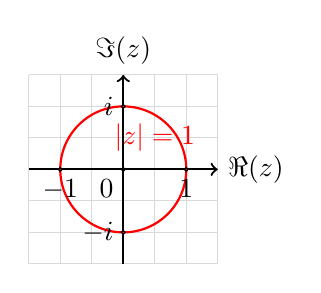
\begin{tikzpicture}[scale=0.8]
\draw[gray!30, step=0.5] (-1.5,-1.5) grid (1.5,1.5);
\draw[thick, ->] (-1.5,0) -- (1.5,0) node[right] {$\Re(z)$};
\draw[thick, ->] (0,-1.5) -- (0,1.5) node[above] {$\Im(z)$};
\draw[fill=black] (0,0) circle (0.03) node[below left] {$0$};
\draw[red, thick] (0,0) circle (1);
\node[red] at (0.5,0.5) {$|z| = 1$};
\draw[fill=red] (1,0) circle (0.03) node[below] {$1$};
\draw[fill=red] (-1,0) circle (0.03) node[below] {$-1$};
\draw[fill=red] (0,1) circle (0.03) node[left] {$i$};
\draw[fill=red] (0,-1) circle (0.03) node[left] {$-i$};
\end{tikzpicture} &
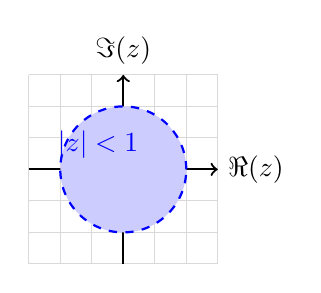
\begin{tikzpicture}[scale=0.8]
\draw[gray!30, step=0.5] (-1.5,-1.5) grid (1.5,1.5);
\draw[thick, ->] (-1.5,0) -- (1.5,0) node[right] {$\Re(z)$};
\draw[thick, ->] (0,-1.5) -- (0,1.5) node[above] {$\Im(z)$};
\draw[fill=black] (0,0) circle (0.03) node[below left] {$0$};
\fill[blue!20] (0,0) circle (1);
\draw[blue, thick, dashed] (0,0) circle (1);
\node[blue] at (-0.4,0.4) {$|z| < 1$};
\end{tikzpicture} \\
\hline
\textbf{(c) Closed unit disk $|z| \leq 1$} & \textbf{(d) Vertical line $\Re(z) = \frac{1}{2}$} \\
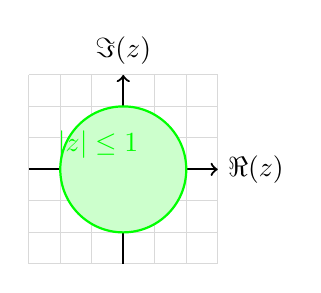
\begin{tikzpicture}[scale=0.8]
\draw[gray!30, step=0.5] (-1.5,-1.5) grid (1.5,1.5);
\draw[thick, ->] (-1.5,0) -- (1.5,0) node[right] {$\Re(z)$};
\draw[thick, ->] (0,-1.5) -- (0,1.5) node[above] {$\Im(z)$};
\draw[fill=black] (0,0) circle (0.03) node[below left] {$0$};
\fill[green!20] (0,0) circle (1);
\draw[green, thick] (0,0) circle (1);
\node[green] at (-0.4,0.4) {$|z| \leq 1$};
\end{tikzpicture} &
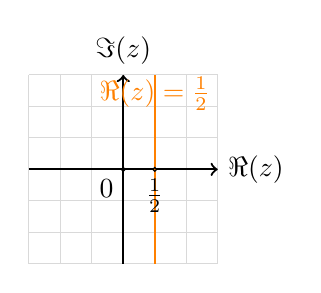
\begin{tikzpicture}[scale=0.8]
\draw[gray!30, step=0.5] (-1.5,-1.5) grid (1.5,1.5);
\draw[thick, ->] (-1.5,0) -- (1.5,0) node[right] {$\Re(z)$};
\draw[thick, ->] (0,-1.5) -- (0,1.5) node[above] {$\Im(z)$};
\draw[fill=black] (0,0) circle (0.03) node[below left] {$0$};
\draw[orange, thick] (0.5,-1.5) -- (0.5,1.5);
\node[orange] at (0.5,1.2) {$\Re(z) = \frac{1}{2}$};
\draw[fill=orange] (0.5,0) circle (0.03) node[below] {$\frac{1}{2}$};
\end{tikzpicture} \\
\hline
\textbf{(e) Horizontal line $\Im(z) = \frac{1}{2}$} & \textbf{(f) Circle $(x-1)^2 + y^2 = 1$} \\
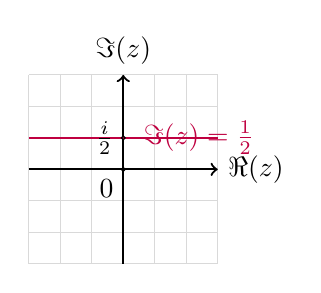
\begin{tikzpicture}[scale=0.8]
\draw[gray!30, step=0.5] (-1.5,-1.5) grid (1.5,1.5);
\draw[thick, ->] (-1.5,0) -- (1.5,0) node[right] {$\Re(z)$};
\draw[thick, ->] (0,-1.5) -- (0,1.5) node[above] {$\Im(z)$};
\draw[fill=black] (0,0) circle (0.03) node[below left] {$0$};
\draw[purple, thick] (-1.5,0.5) -- (1.5,0.5);
\node[purple] at (1.2,0.5) {$\Im(z) = \frac{1}{2}$};
\draw[fill=purple] (0,0.5) circle (0.03) node[left] {$\frac{i}{2}$};
\end{tikzpicture} &
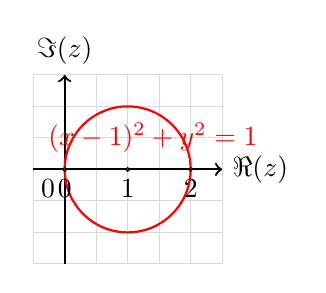
\begin{tikzpicture}[scale=0.8]
\draw[gray!30, step=0.5] (-0.5,-1.5) grid (2.5,1.5);
\draw[thick, ->] (-0.5,0) -- (2.5,0) node[right] {$\Re(z)$};
\draw[thick, ->] (0,-1.5) -- (0,1.5) node[above] {$\Im(z)$};
\draw[fill=black] (0,0) circle (0.03) node[below left] {$0$};
\draw[red, thick] (1,0) circle (1);
\node[red] at (1.4,0.5) {$(x-1)^2 + y^2 = 1$};
\draw[fill=red] (1,0) circle (0.03) node[below] {$1$};
\draw[fill=red] (0,0) circle (0.03) node[below] {$0$};
\draw[fill=red] (2,0) circle (0.03) node[below] {$2$};
\end{tikzpicture} \\
\hline
\end{tabular}
\end{center}\qed


\begin{problembox}[1.31: Equilateral Triangle on the Unit Circle]
\begin{problemstatement}
Given three complex numbers \( z_1, z_2, z_3 \) such that \( |z_1| = |z_2| = |z_3| = 1 \) and \( z_1 + z_2 + z_3 = 0 \), show that these numbers are vertices of an equilateral triangle inscribed in the unit circle with center at the origin.
\end{problemstatement}
\end{problembox}

\noindent\textbf{Strategy:} Use the fact that the sum of three unit complex numbers equals zero to show they must be the cube roots of unity (rotated), which form an equilateral triangle. Verify that the angles differ by $2\pi/3$ and the sum condition is satisfied.

\bigskip\noindent\textbf{Solution:}
Since \( |z_i| = 1 \), each \( z_i = e^{i\theta_i} \) lies on the unit circle. Given \( z_1 + z_2 + z_3 = 0 \), we need to show they form an equilateral triangle. Consider the angles \( \theta_1, \theta_2, \theta_3 \). The sum condition implies:
\[
e^{i\theta_1} + e^{i\theta_2} + e^{i\theta_3} = 0.
\]
For three points on the unit circle to form an equilateral triangle, their arguments must differ by \( 120^\circ = \frac{2\pi}{3} \). Assume:
\[
z_1 = e^{i\theta}, \quad z_2 = e^{i(\theta + \frac{2\pi}{3})}, \quad z_3 = e^{i(\theta + \frac{4\pi}{3})}.
\]
Check the sum:
\[
e^{i\theta} + e^{i(\theta + \frac{2\pi}{3})} + e^{i(\theta + \frac{4\pi}{3})} = e^{i\theta} \left( 1 + e^{i\frac{2\pi}{3}} + e^{i\frac{4\pi}{3}} \right).
\]
Since \( e^{i\frac{2\pi}{3}} = -\frac{1}{2} + i\frac{\sqrt{3}}{2} \), \( e^{i\frac{4\pi}{3}} = -\frac{1}{2} - i\frac{\sqrt{3}}{2} \), we have:
\[
1 + e^{i\frac{2\pi}{3}} + e^{i\frac{4\pi}{3}} = 1 + \left(-\frac{1}{2} + i\frac{\sqrt{3}}{2}\right) + \left(-\frac{1}{2} - i\frac{\sqrt{3}}{2}\right) = 0.
\]
The angles \( \theta, \theta + \frac{2\pi}{3}, \theta + \frac{4\pi}{3} \) are spaced \( \frac{2\pi}{3} \) apart, forming an equilateral triangle. Any three points with \( |z_i| = 1 \) and sum zero are rotations of the cube roots of unity, ensuring an equilateral triangle.

\textbf{Visualization:}
\begin{center}
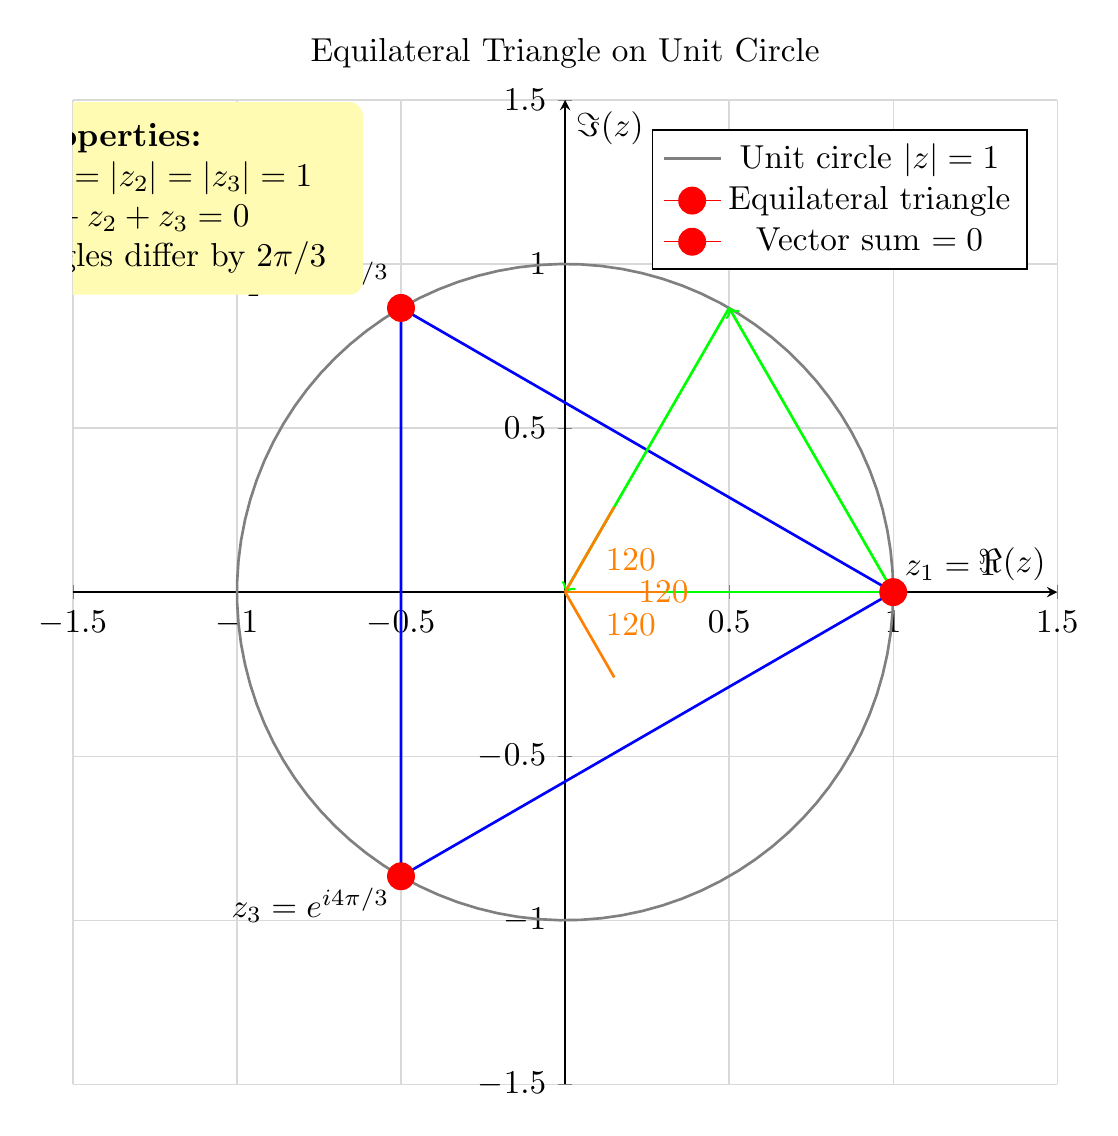
\begin{tikzpicture}[scale=1.2]
\begin{axis}[
    width=12cm,
    height=12cm,
    xlabel={$\Re(z)$},
    ylabel={$\Im(z)$},
    title={Equilateral Triangle on Unit Circle},
    xmin=-1.5, xmax=1.5,
    ymin=-1.5, ymax=1.5,
    grid=major,
    grid style={gray!30},
    axis lines=middle,
    axis equal,
    legend pos=north east
]

% Unit circle
\addplot[gray, thick, samples=100, domain=0:360] ({cos(x)}, {sin(x)});
\addlegendentry{Unit circle $|z| = 1$}

% Equilateral triangle vertices (cube roots of unity)
\addplot[red, mark=*, mark size=4pt] coordinates {(1,0)};
\node[above right] at (axis cs:1,0) {$z_1 = 1$};

\addplot[red, mark=*, mark size=4pt] coordinates {(-0.5,0.866)};
\node[above left] at (axis cs:-0.5,0.866) {$z_2 = e^{i2\pi/3}$};

\addplot[red, mark=*, mark size=4pt] coordinates {(-0.5,-0.866)};
\node[below left] at (axis cs:-0.5,-0.866) {$z_3 = e^{i4\pi/3}$};

% Draw the triangle
\addplot[blue, thick] coordinates {(1,0) (-0.5,0.866) (-0.5,-0.866) (1,0)};
\addlegendentry{Equilateral triangle}

% Show the sum equals zero
\addplot[green, thick, ->] coordinates {(0,0) (1,0)};
\addplot[green, thick, ->] coordinates {(1,0) (0.5,0.866)};
\addplot[green, thick, ->] coordinates {(0.5,0.866) (0,0)};
\addlegendentry{Vector sum $= 0$}

% Add angle markers
\draw[orange, thick] (axis cs:0,0) -- (axis cs:0.3,0);
\draw[orange, thick] (axis cs:0,0) -- (axis cs:0.15,0.26);
\draw[orange, thick] (axis cs:0,0) -- (axis cs:0.15,-0.26);
\node[orange] at (axis cs:0.2,0.1) {$120°$};
\node[orange] at (axis cs:0.2,-0.1) {$120°$};
\node[orange] at (axis cs:0.3,0) {$120°$};

% Add text explaining the properties
\node[fill=yellow!30, rounded corners, inner sep=5pt] at (axis cs:-1.2,1.2) {
    \begin{tabular}{l}
    \textbf{Properties:} \\
    $|z_1| = |z_2| = |z_3| = 1$ \\
    $z_1 + z_2 + z_3 = 0$ \\
    Angles differ by $2\pi/3$
    \end{tabular}
};

\end{axis}
\end{tikzpicture}
\end{center}

This visualization shows the equilateral triangle formed by the cube roots of unity on the unit circle. The green vectors show how the sum of the three complex numbers equals zero, and the orange angle markers show the $120°$ spacing between vertices.\qed


\begin{problembox}[1.32: Inequality with Complex Numbers]
\begin{problemstatement}
If \( a \) and \( b \) are complex numbers, prove:
\begin{enumerate}[label=\alph*)]
\item \( |a - b|^2 \leq (1 + |a|^2)(1 + |b|^2) \),
\item If \( a \neq 0 \), then \( |a + b| = |a| + |b| \) if and only if \( \frac{b}{a} \) is real and nonnegative.
\end{enumerate}
\end{problemstatement}
\end{problembox}

\noindent\textbf{Strategy:} For part (a), we'll expand both sides and show that the difference is non-negative. For part (b), we'll use the fact that equality in the triangle inequality occurs when the complex numbers are collinear and point in the same direction.

\bigskip\noindent\textbf{Solution:}
\begin{enumerate}[label=\alph*)]
\item Compute:
\[
|a - b|^2 = (a - b)(\overline{a - b}) = |a|^2 + |b|^2 - a\overline{b} - \overline{a}b.
\]
Consider the right-hand side:
\[
(1 + |a|^2)(1 + |b|^2) = 1 + |a|^2 + |b|^2 + |a|^2 |b|^2.
\]
Evaluate:
\[
(1 + |a|^2)(1 + |b|^2) - |a - b|^2 = 1 + |a b|^2 + a\overline{b} + \overline{a}b = 1 + |a b|^2 + 2\Re(a\overline{b}).
\]
Since \( |a b|^2 \geq 0 \), \( \Re(a\overline{b}) \geq -|a b| \):
\[
1 + |a b|^2 + 2\Re(a\overline{b}) \geq 1 + |a b|^2 - 2|a b| = (1 - |a b|)^2 \geq 0.
\]
Thus, \( |a - b|^2 \leq (1 + |a|^2)(1 + |b|^2) \).
\item For \( |a + b| = |a| + |b| \), the triangle inequality requires \( a, b \) collinear in the same direction. Let \( b = ka \), \( k \in \mathbb{R}_{\geq 0} \):
\[
|a + b| = |a + ka| = |a|(1 + k) = |a| + |b|.
\]
Thus, \( \frac{b}{a} = k \geq 0 \). Conversely, if \( |a + b| = |a| + |b| \), then \( a\overline{b} + \overline{a}b = 2|a||b| \), so \( \frac{b}{a} \) is real and nonnegative.
\end{enumerate}\qed


\begin{problembox}[1.33: Equality Condition for Complex Difference]
\begin{problemstatement}
If \( a \) and \( b \) are complex numbers, prove that
\[
|a - b| = |1 - \overline{a}b|
\]
if and only if \( |a| = 1 \) or \( |b| = 1 \). For which \( a \) and \( b \) is the inequality \( |a - b| < |1 - \overline{a}b| \) valid?
\end{problemstatement}
\end{problembox}

\noindent\textbf{Strategy:} We will compute the difference $|a - b|^2 - |1 - \overline{a}b|^2$ and show that it factors as $(r^2 - 1)(s^2 - 1)$ where $r = |a|$ and $s = |b|$. This will allow us to determine when equality holds and when the inequality is valid.

\bigskip\noindent\textbf{Solution:}
Let \( |a| = r \), \( |b| = s \). Compute:
\[
|a - b|^2 = r^2 + s^2 - a\overline{b} - \overline{a}b, \quad |1 - \overline{a}b|^2 = 1 + r^2 s^2 - a\overline{b} - \overline{a}b.
\]
Thus:
\[
|a - b|^2 - |1 - \overline{a}b|^2 = r^2 + s^2 - 1 - r^2 s^2 = (r^2 - 1)(s^2 - 1).
\]
Equality holds when:
\[
(r^2 - 1)(s^2 - 1) = 0 \implies r = 1 \text{ or } s = 1.
\]
For the inequality:
\[
(r^2 - 1)(s^2 - 1) < 0 \implies (r^2 < 1 \text{ and } s^2 > 1) \text{ or } (r^2 > 1 \text{ and } s^2 < 1).
\]
Thus, equality holds if \( |a| = 1 \) or \( |b| = 1 \); the inequality holds when one modulus is less than 1 and the other is greater than 1.\qed


\begin{problembox}[1.34: Complex Circle in the Plane]
\begin{problemstatement}
If \( a \) and \( c \) are real constants, \( b \) is complex, show that the equation
\[
az\overline{z} + bz + \overline{b} \overline{z} + c = 0 \qquad (a \ne 0, z = x + iy)
\]
represents a circle in the \( xy \)-plane.
\end{problemstatement}
\end{problembox}

\noindent\textbf{Strategy:} We will substitute $z = x + iy$ and $\overline{z} = x - iy$ into the equation, then use the fact that $z\overline{z} = x^2 + y^2$ and $bz + \overline{b}\overline{z} = 2\Re(bz)$ to show that the equation reduces to the general form of a circle.

\bigskip\noindent\textbf{Solution:}
Let \( z = x + iy \), \( \overline{z} = x - iy \), then \( z \overline{z} = x^2 + y^2 \), \( bz + \overline{b} \overline{z} = 2 \Re(b z) \). Hence the equation becomes:
\[
a(x^2 + y^2) + 2 \Re(b z) + c = 0.
\]
This is the general form of a circle in \( \mathbb{R}^2 \).\qed


\begin{problembox}[1.35: Argument of a Complex Number via Arctangent]
\begin{problemstatement}
Recall the definition of the inverse tangent: given a real number \( t \), \( \tan^{-1}(t) \) is the unique real number \( \theta \) satisfying:
\[
-\frac{\pi}{2} < \theta < \frac{\pi}{2}, \quad \text{and} \quad \tan \theta = t.
\]
If \( z = x + iy \), show that:
\begin{enumerate}[label=\alph*)]
\item \( \arg(z) = \tan^{-1}\left( \frac{y}{x} \right) \), if \( x > 0 \),
\item \( \arg(z) = \tan^{-1}\left( \frac{y}{x} \right) + \pi \), if \( x < 0 \), \( y \geq 0 \),
\item \( \arg(z) = \tan^{-1}\left( \frac{y}{x} \right) - \pi \), if \( x < 0 \), \( y < 0 \),
\item \( \arg(z) = \frac{\pi}{2} \), if \( x = 0, y > 0 \); \quad \( \arg(z) = -\frac{\pi}{2} \), if \( x = 0, y < 0 \).
\end{enumerate}
\end{problemstatement}
\end{problembox}

\noindent\textbf{Strategy:} We will use the relationship between the argument of a complex number and the quadrant it lies in. The principal value of $\tan^{-1}$ gives angles in $(-\pi/2, \pi/2]$, so we need to adjust for different quadrants to get the correct argument in $(-\pi, \pi]$.

\bigskip\noindent\textbf{Solution:}
For \( z = x + iy \), \( \arg(z) \) is the angle \( \theta \in (-\pi, \pi] \) such that \( z = |z| e^{i\theta} \).
\begin{enumerate}[label=\alph*)]
\item If \( x > 0 \), \( z \) is in Quadrant I or IV, and \( \tan \theta = \frac{y}{x} \), so \( \theta = \tan^{-1}\left( \frac{y}{x} \right) \).
\item If \( x < 0 \), \( y \geq 0 \), \( z \) is in Quadrant II. \( \tan^{-1}\left( \frac{y}{x} \right) \in (-\frac{\pi}{2}, 0] \), so add \( \pi \) to get \( \theta \in (\frac{\pi}{2}, \pi] \).
\item If \( x < 0 \), \( y < 0 \), \( z \) is in Quadrant III. \( \tan^{-1}\left( \frac{y}{x} \right) \in (0, \frac{\pi}{2}] \), so subtract \( \pi \) to get \( \theta \in (-\pi, -\frac{\pi}{2}] \).
\item If \( x = 0 \), \( z = iy \). If \( y > 0 \), \( \theta = \frac{\pi}{2} \); if \( y < 0 \), \( \theta = -\frac{\pi}{2} \).
\end{enumerate}\qed


\begin{problembox}[1.36: Pseudo-Ordering on Complex Numbers]
\begin{problemstatement}
Define the following pseudo-ordering on complex numbers: $z_1 < z_2$ if $|z_1| < |z_2|$, or if $|z_1|=|z_2|$ and $\arg(z_1) < \arg(z_2)$. Which of Axioms 6,7,8,9 are satisfied by this relation?
\end{problemstatement}
\end{problembox}

\noindent\textbf{Strategy:} We will examine each axiom individually, testing whether the pseudo-ordering satisfies the properties of trichotomy, translation invariance, multiplication invariance, and transitivity. We'll provide counterexamples where axioms fail.

\begin{itemize}
    \item \textbf{Axiom 6 (Trichotomy):} For any $z_1, z_2 \in \mathbb{C}$, we can compare their moduli. Exactly one of $|z_1| < |z_2|$, $|z_1| > |z_2|$, or $|z_1| = |z_2|$ holds. If $|z_1| = |z_2|$, we compare their principal arguments, for which trichotomy holds on $(-\pi, \pi]$. Thus, exactly one of $z_1 < z_2$, $z_2 < z_1$, or $z_1 = z_2$ is true. This axiom is \textbf{satisfied}.

    \item \textbf{Axiom 9 (Transitivity):} If $z_1 < z_2$ and $z_2 < z_3$, the transitivity of the $<$ relation on the real numbers for both the moduli and the arguments ensures that $z_1 < z_3$. This axiom is \textbf{satisfied}.

    \item \textbf{Axiom 7 (Translation Invariance):} This axiom states that if $z_1 < z_2$, then $z_1 + z < z_2 + z$ for any $z \in \mathbb{C}$. This axiom is \textbf{not satisfied}.
    
    \textbf{Counterexample:} Let $z_1 = 1$ and $z_2 = 2$. According to the ordering, $z_1 < z_2$ because $|z_1|=1 < |z_2|=2$.
    Now, let $z = -2$.
    Then $z_1 + z = 1 + (-2) = -1$.
    And $z_2 + z = 2 + (-2) = 0$.
    We must compare $z_1+z = -1$ and $z_2+z=0$.
    We have $|-1|=1$ and $|0|=0$. Since $|0| < |-1|$, we have $0 < -1$ in this pseudo-ordering.
    So, $z_2 + z < z_1 + z$. The order relation was reversed, which violates the axiom.

    \item \textbf{Axiom 8 (Multiplication):} This axiom states that if $z_1 < z_2$ and $z > 0$, then $z_1 z < z_2 z$. Let us define $z>0$ to mean $0<z$. This holds for any $z \neq 0$. This axiom is also \textbf{not satisfied}.
    
    \textbf{Counterexample:} Let $z_1 = e^{i\pi} = -1$ and $z_2 = e^{-i\pi/2} = -i$.
    We have $|z_1| = |z_2| = 1$. The arguments are $\arg(z_1) = \pi$ and $\arg(z_2) = -\pi/2$. Since $-\pi/2 < \pi$, we have $z_2 < z_1$.
    Now, let $z = i$. Since $i \neq 0$, $z$ is a "positive" number under this definition.
    Then $z_1 z = (-1)(i) = -i$.
    And $z_2 z = (-i)(i) = 1$.
    We must compare $z_1 z = -i$ and $z_2 z = 1$.
    We have $|-i|=1$ and $|1|=1$. The arguments are $\arg(-i) = -\pi/2$ and $\arg(1) = 0$. Since $-\pi/2 < 0$, we have $-i < 1$.
    So, $z_1 z < z_2 z$. The order relation was reversed from $z_2 < z_1$ to $z_1 z < z_2 z$. The axiom is violated.
\end{itemize}
\textbf{Conclusion:} Axioms 6 and 9 are satisfied; Axiom 7 and 8 is not applicable.



\begin{problembox}[1.37: Order Axioms and Lexicographic Ordering on $\mathbb{R}^2$]
\begin{problemstatement}
Define a pseudo-ordering on ordered pairs \((x_1, y_1) < (x_2, y_2)\) if either
\begin{enumerate}[label=(\roman*)]
\item \(x_1 < x_2\), or
\item \(x_1 = x_2\) and \(y_1 < y_2\).
\end{enumerate}
Which of Axioms 6, 7, 8, 9 are satisfied by this relation?
\end{problemstatement}
\end{problembox}

\noindent\textbf{Strategy:} We will examine each axiom for the lexicographic ordering on $\mathbb{R}^2$. This ordering compares first coordinates, then second coordinates if the first coordinates are equal, which should preserve most of the standard ordering properties.

\bigskip\noindent\textbf{Solution:}
\begin{itemize}
\item \textbf{Axiom 6: Trichotomy.} For any \( (x_1, y_1), (x_2, y_2) \), if \( x_1 < x_2 \), then \( (x_1, y_1) < (x_2, y_2) \); if \( x_1 > x_2 \), then \( (x_2, y_2) < (x_1, y_1) \); if \( x_1 = x_2 \), compare \( y_1, y_2 \). Exactly one holds. Satisfied.
\item \textbf{Axiom 7: Translation Invariance.} If \( (x_1, y_1) < (x_2, y_2) \), add \( (u, v) \): if \( x_1 < x_2 \), then \( x_1 + u < x_2 + u \); if \( x_1 = x_2 \), then \( y_1 < y_2 \implies y_1 + v < y_2 + v \). Satisfied.
\item \textbf{Axiom 8: Multiplication.} Not applicable, as \( \mathbb{R}^2 \) lacks scalar multiplication.
\item \textbf{Axiom 9: Transitivity.} If \( (x_1, y_1) < (x_2, y_2) \), \( (x_2, y_2) < (x_3, y_3) \), lexicographic order ensures \( (x_1, y_1) < (x_3, y_3) \). Satisfied.
\end{itemize}
\textbf{Conclusion:} Axioms 6, 7, and 9 are satisfied; Axiom 8 is not applicable.\qed


\begin{problembox}[1.38: Argument of a Quotient Using Theorem 1.48]
\begin{problemstatement}
State and prove a theorem analogous to Theorem 1.48, expressing \( \arg\left( \frac{z_1}{z_2} \right) \) in terms of \( \arg(z_1) \) and \( \arg(z_2) \).
\end{problemstatement}
\end{problembox}

\noindent\textbf{Strategy:} We will use the fact that $\frac{z_1}{z_2} = z_1 z_2^{-1}$ and apply Theorem 1.48 to the product, using the property that $\arg(z_2^{-1}) = -\arg(z_2)$.

\bigskip\noindent\textbf{Solution:}
\textbf{Theorem:} If \( z_1, z_2 \neq 0 \), then:
\[
\arg\left( \frac{z_1}{z_2} \right) = \arg(z_1) - \arg(z_2) + 2\pi n(z_1, z_2^{-1}),
\]
where \( n(z_1, z_2^{-1}) \) adjusts the argument to \( (-\pi, \pi] \).

\bigskip\noindent\textbf{Solution:}
Since \( \frac{z_1}{z_2} = z_1 z_2^{-1} \), and \( \arg(z_2^{-1}) = -\arg(z_2) \), apply Theorem 1.48:

\begin{align*}
\arg(z_1 z_2^{-1}) =& \arg(z_1) + \arg(z_2^{-1}) + 2\pi n(z_1, z_2^{-1}) \\
=& \arg(z_1) - \arg(z_2) + 2\pi n(z_1, z_2^{-1}).
\end{align*}\qed


\begin{problembox}[1.39: Logarithm of a Quotient Using Theorem 1.54]
\begin{problemstatement}
State and prove a theorem analogous to Theorem 1.54, expressing \( \log\left( \frac{z_1}{z_2} \right) \) in terms of \( \log(z_1) \) and \( \log(z_2) \).
\end{problemstatement}
\end{problembox}

\noindent\textbf{Strategy:} We will use the fact that $\frac{z_1}{z_2} = z_1 z_2^{-1}$ and apply Theorem 1.54 to the product, using the property that $\log(z_2^{-1}) = -\log(z_2)$.

\bigskip\noindent\textbf{Solution:}
\textbf{Theorem:} If \( z_1, z_2 \neq 0 \), then:
\[
\log\left( \frac{z_1}{z_2} \right) = \log z_1 - \log z_2 + 2\pi i n(z_1, z_2^{-1}).
\]
\bigskip\noindent\textbf{Solution:}
Since \( \frac{z_1}{z_2} = z_1 z_2^{-1} \), apply Theorem 1.54:
\begin{align*}
\log(z_1 z_2^{-1}) =& \log z_1 + \log(z_2^{-1}) + 2\pi i n(z_1, z_2^{-1}) \\
=& \log z_1 - \log z_2 + 2\pi i n(z_1, z_2^{-1}).
\end{align*}\qed


\begin{problembox}[1.40: Roots of Unity and Polynomial Identity]
\begin{problemstatement}
Prove that the \( n \)th roots of 1 are given by \( \alpha, \alpha^2, \ldots, \alpha^n \), where \( \alpha = e^{2\pi i/n} \), and that these roots \( \ne 1 \) satisfy the equation
\[
1 + x + x^2 + \cdots + x^{n-1} = 0.
\]
\end{problemstatement}
\end{problembox}

\noindent\textbf{Strategy:} We will use the fact that the $n$th roots of unity are the solutions to $x^n - 1 = 0$, and use the factorization $\frac{x^n - 1}{x - 1} = 1 + x + x^2 + \cdots + x^{n-1}$ to show that all roots except $x = 1$ satisfy the given equation.

\bigskip\noindent\textbf{Solution:}
Let \( \alpha = e^{2\pi i/n} \). Then \( \alpha^n = 1 \), so it's a root of \( x^n - 1 = 0 \). Also,
\[
\frac{1 - \alpha^n}{1 - \alpha} = 0 \Rightarrow 1 + \alpha + \cdots + \alpha^{n-1} = 0 \quad \text{for } \alpha \ne 1.
\]\qed


\begin{problembox}[1.41: Inequalities and Boundedness of cos z]
\begin{problemstatement}
\begin{enumerate}[label=\alph*)]
\item Prove that \( |z^i| < e^{\pi} \) for all complex \( z \ne 0 \).
\item Prove that there is no constant \( M > 0 \) such that \( |\cos z| < M \) for all complex \( z \).
\end{enumerate}
\end{problemstatement}
\end{problembox}

\noindent\textbf{Strategy:} For part (a), we'll use the definition $z^i = e^{i\log z}$ and analyze the modulus in terms of the argument. For part (b), we'll use the fact that $\cos(iy) = \cosh y$ which grows exponentially as $y \to \infty$.

\bigskip\noindent\textbf{Solution:}
\begin{enumerate}[label=\alph*)]
\item For \( z = re^{i\theta} \), \( z^i = e^{i(\ln r + i\theta)} = e^{-\theta} e^{i \ln r} \), so \( |z^i| = e^{-\theta} \). Since \( \theta \in (-\pi, \pi] \), \( |z^i| \leq e^{\pi} \), strict unless \( \theta = -\pi \).
\item For \( z = iy \), \( \cos(iy) = \cosh y \), which is unbounded as \( |y| \to \infty \). Thus, no \( M > 0 \) exists.
\end{enumerate}\qed


\begin{problembox}[1.42: Complex Exponential via Real and Imaginary Parts]
\begin{problemstatement}
If \( w = u + iv \), where \( u \) and \( v \) are real, show that
\[
z^w = e^{u \log |z| - v \arg(z)} \cdot e^{i[v \log |z| + u \arg(z)]}.
\]
\end{problemstatement}
\end{problembox}

\noindent\textbf{Strategy:} We will use the definition $z^w = e^{w \log z}$ and expand the product $(u + iv)(\log |z| + i \arg z)$ to separate the real and imaginary parts.

\bigskip\noindent\textbf{Solution:}
For \( z^w = e^{w \log z} \), where \( \log z = \log |z| + i \arg z \):
\[
w \log z = (u + iv)(\log |z| + i \arg z) = (u \log |z| - v \arg z) + i(v \log |z| + u \arg z).
\]
Thus:
\[
z^w = e^{u \log |z| - v \arg z} e^{i(v \log |z| + u \arg z)}.
\]\qed


\begin{problembox}[1.43: Logarithmic Identities for Complex Powers]
\begin{problemstatement}
\begin{enumerate}[label=\alph*)]
\item Prove that \( \log(z^w) = w \log z + 2\pi i n \), where \( n \) is an integer.
\item Prove that \( (z^w)^\alpha = z^{w\alpha} e^{2\pi i n \alpha} \), where \( n \) is an integer.
\end{enumerate}
\end{problemstatement}
\end{problembox}

\noindent\textbf{Strategy:} For part (a), we'll use the definition $z^w = e^{w \log z}$ and the fact that $\log(e^w) = w + 2\pi i n$. For part (b), we'll use the result from part (a) and the definition of complex exponentiation.

\bigskip\noindent\textbf{Solution:}
\begin{enumerate}[label=\alph*)]
\item Since \( z^w = e^{w \log z} \):
\[
\log(z^w) = \log(e^{w \log z}) = w \log z + 2\pi i n.
\]
\item Compute:
\[
(z^w)^\alpha = e^{\alpha \log(z^w)} = e^{\alpha(w \log z + 2\pi i n)} = z^{w\alpha} e^{2\pi i n \alpha}.
\]
\end{enumerate}\qed


\begin{problembox}[1.44: Conditions for De Moivre's Formula]
\begin{problemstatement}
\begin{enumerate}[label=\roman*)]
\item If \( \theta \) and \( a \) are real numbers, \( -\pi < \theta \leq +\pi \), prove that
\[
(\cos \theta + i \sin \theta)^a = \cos(a\theta) + i \sin(a\theta).
\]
\item Show that, in general, the restriction \( -\pi < \theta \leq +\pi \) is necessary in (i) by taking \( \theta = -\pi \), \( a = \tfrac{1}{2} \).
\item If \( a \) is an integer, show that the formula in (i) holds without any restriction on \( \theta \). In this case it is known as De Moivre's theorem.
\end{enumerate}
\end{problemstatement}
\end{problembox}

\noindent\textbf{Strategy:} We will use the fact that $\cos \theta + i \sin \theta = e^{i\theta}$ and the definition of complex exponentiation. For part (b), we'll provide a specific counterexample. For part (c), we'll use the fact that integer powers don't have branch cut issues.

\bigskip\noindent\textbf{Solution:}
\begin{enumerate}[label=\roman*)]
\item Since \( \cos \theta + i \sin \theta = e^{i\theta} \):
\[
(\cos \theta + i \sin \theta)^a = (e^{i\theta})^a = e^{i a \theta} = \cos(a\theta) + i \sin(a\theta).
\]
\item For \( \theta = -\pi \), \( a = \frac{1}{2} \):
\[
(-1)^{1/2} = i, \quad \text{but} \quad \cos\left(\frac{-\pi}{2}\right) + i \sin\left(\frac{-\pi}{2}\right) = -i.
\]
The restriction ensures the principal branch.
\item For integer \( a \), \( (e^{i\theta})^a = e^{i a \theta} \), and multiples of \( 2\pi \) cancel, so the formula holds for all \( \theta \).
\end{enumerate}\qed


\begin{problembox}[1.45: Deriving Trigonometric Identities from De Moivre's Theorem]
\begin{problemstatement}
Use De Moivre's theorem (Exercise 1.44) to derive the trigonometric identities
\[
\sin 3\theta = 3 \cos^2 \theta \sin \theta - \sin^3 \theta,
\]
\[
\cos 3\theta = \cos^3 \theta - 3 \cos \theta \sin^2 \theta,
\]
valid for real \( \theta \). Are these valid when \( \theta \) is complex?
\end{problemstatement}
\end{problembox}

\noindent\textbf{Strategy:} We will use De Moivre's theorem to expand $(\cos \theta + i \sin \theta)^3$, then equate the real and imaginary parts to obtain the desired identities. Since $\cos z$ and $\sin z$ are analytic functions, these identities extend to complex $\theta$.

\bigskip\noindent\textbf{Solution:}
By De Moivre's theorem:
\[
(\cos \theta + i \sin \theta)^3 = \cos 3\theta + i \sin 3\theta.
\]
Expand:
\[
\cos^3 \theta + 3i \cos^2 \theta \sin \theta - 3 \cos \theta \sin^2 \theta - i \sin^3 \theta.
\]
Equate parts:
\[
\cos 3\theta = \cos^3 \theta - 3 \cos \theta \sin^2 \theta, \quad \sin 3\theta = 3 \cos^2 \theta \sin \theta - \sin^3 \theta.
\]
These hold for complex \( \theta \), as \( \cos z \) and \( \sin z \) are analytic.\qed


\begin{problembox}[1.46: Tangent of Complex Numbers]
\begin{problemstatement}
Define \( \tan z = \frac{\sin z}{\cos z} \), and show that for \( z = x + iy \),
\[
\tan z = \frac{\sin 2x + i \sinh 2y}{\cos 2x + \cosh 2y}.
\]
\end{problemstatement}
\end{problembox}

\noindent\textbf{Strategy:} We will use the expressions for $\sin z$ and $\cos z$ in terms of real and imaginary parts, then rationalize the denominator by multiplying by the complex conjugate and simplify using trigonometric and hyperbolic identities.

\bigskip\noindent\textbf{Solution:}
For \( z = x + iy \):
\[
\sin z = \sin x \cosh y + i \cos x \sinh y, \quad \cos z = \cos x \cosh y - i \sin x \sinh y.
\]
Compute:
\[
\tan z = \frac{\sin x \cosh y + i \cos x \sinh y}{\cos x \cosh y - i \sin x \sinh y}.
\]
Multiply by the conjugate of the denominator:
\[
N = (\sin x \cosh y + i \cos x \sinh y)(\cos x \cosh y + i \sin x \sinh y) = \sin 2x + i \sinh 2y,
\]
\[
D = (\cos x \cosh y)^2 + (\sin x \sinh y)^2 = \frac{1}{2}(\cos 2x + \cosh 2y).
\]
Thus:
\[
\tan z = \frac{\sin 2x + i \sinh 2y}{\cos 2x + \cosh 2y}.
\]\qed


\begin{problembox}[1.47: Solving Cosine Equation]
\begin{problemstatement}
Let \( w \) be a complex number. If \( w \ne \pm 1 \), show that there exist two values \( z = x + iy \) with \( \cos z = w \) and \( -\pi < x \leq \pi \). Find such \( z \) when \( w = i \) and \( w = 2 \).
\end{problemstatement}
\end{problembox}

\noindent\textbf{Strategy:} We will use the expression for $\cos z$ in terms of real and imaginary parts, then solve the resulting system of equations for $x$ and $y$. We'll provide specific solutions for the given values of $w$.

\bigskip\noindent\textbf{Solution:}
For \( z = x + iy \), \( \cos z = \cos x \cosh y - i \sin x \sinh y = w = u + iv \). Solve:
\[
\cos x \cosh y = u, \quad -\sin x \sinh y = v.
\]
Square and add:
\[
\sin^2 x = \sinh^2 y + 1 - u^2 - v^2.
\]
Since \( w \neq \pm 1 \), solutions exist, with two \( x \) in \( (-\pi, \pi] \).

\textbf{Case 1: \( w = i \).} \( u = 0 \), \( v = 1 \):
\[
\cos x \cosh y = 0 \implies x = \pm \frac{\pi}{2}.
\]
For \( x = \frac{\pi}{2} \), \( \sinh y = -1 \implies y = -\ln(1 + \sqrt{2}) \).
For \( x = -\frac{\pi}{2} \), \( \sinh y = 1 \implies y = \ln(1 + \sqrt{2}) \).
Solutions: \( z_1 = \frac{\pi}{2} - i \ln(1 + \sqrt{2}) \), \( z_2 = -\frac{\pi}{2} + i \ln(1 + \sqrt{2}) \).

\textbf{Case 2: \( w = 2 \).} \( u = 2 \), \( v = 0 \):
\[
\cos x \cosh y = 2, \quad \sin x \sinh y = 0.
\]
Thus, \( x = 0 \), \( \cosh y = 2 \implies y = \pm \ln(2 + \sqrt{3}) \).
Solutions: \( z_1 = i \ln(2 + \sqrt{3}) \), \( z_2 = -i \ln(2 + \sqrt{3}) \).

\textbf{Visualization:}
\begin{center}
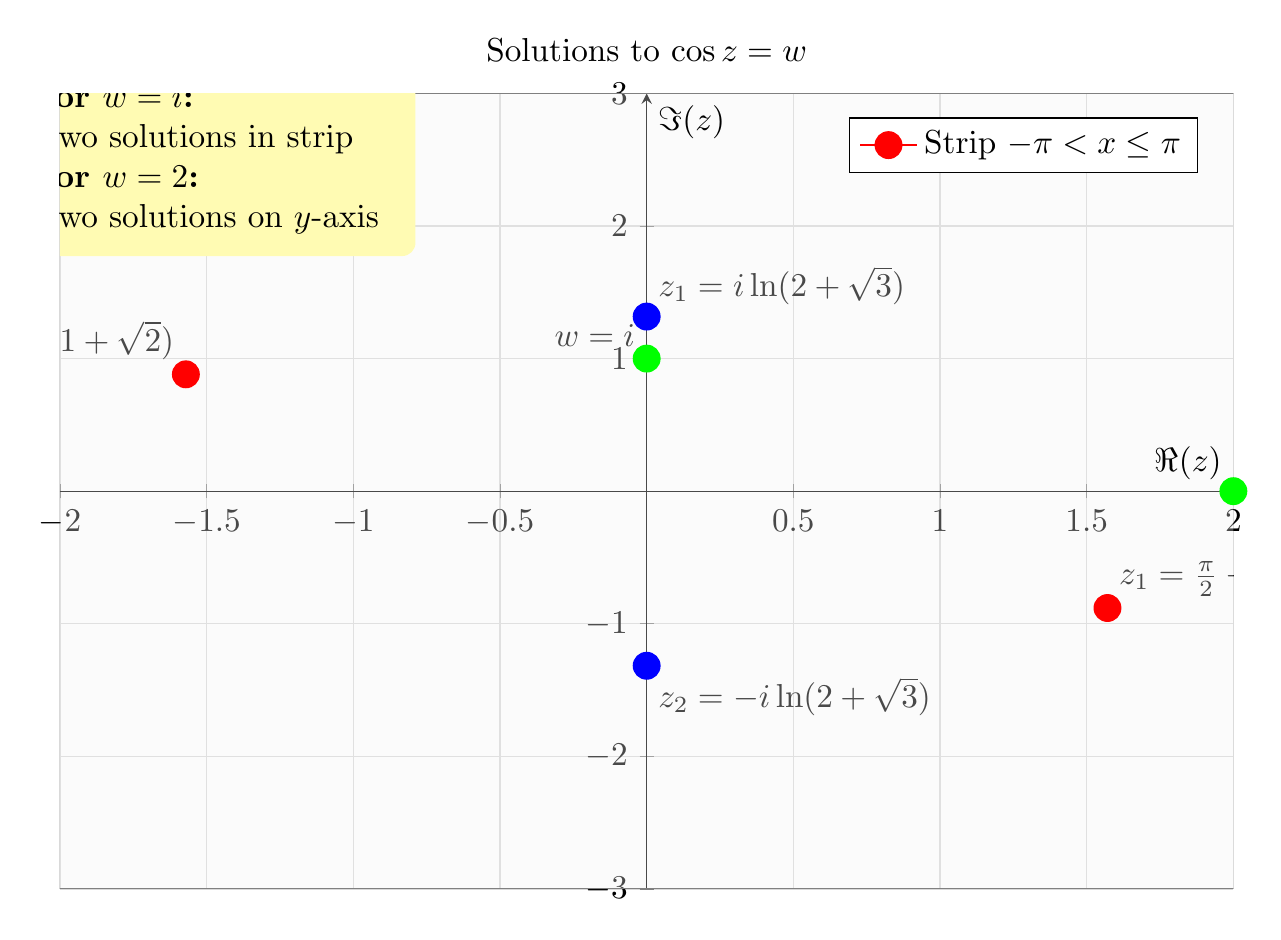
\begin{tikzpicture}[scale=1.2]
\begin{axis}[
    width=14cm,
    height=10cm,
    xlabel={$\Re(z)$},
    ylabel={$\Im(z)$},
    title={Solutions to $\cos z = w$},
    xmin=-2, xmax=2,
    ymin=-3, ymax=3,
    grid=major,
    grid style={gray!30},
    axis lines=middle,
    legend pos=north east
]

% Solutions for w = i
\addplot[red, mark=*, mark size=4pt] coordinates {(1.5708,-0.8814)};
\node[above right] at (axis cs:1.5708,-0.8814) {$z_1 = \frac{\pi}{2} - i\ln(1+\sqrt{2})$};

\addplot[red, mark=*, mark size=4pt] coordinates {(-1.5708,0.8814)};
\node[above left] at (axis cs:-1.5708,0.8814) {$z_2 = -\frac{\pi}{2} + i\ln(1+\sqrt{2})$};

% Solutions for w = 2
\addplot[blue, mark=*, mark size=4pt] coordinates {(0,1.317)};
\node[above right] at (axis cs:0,1.317) {$z_1 = i\ln(2+\sqrt{3})$};

\addplot[blue, mark=*, mark size=4pt] coordinates {(0,-1.317)};
\node[below right] at (axis cs:0,-1.317) {$z_2 = -i\ln(2+\sqrt{3})$};

% Mark the values of w
\addplot[green, mark=*, mark size=4pt] coordinates {(0,1)};
\node[above left] at (axis cs:0,1) {$w = i$};

\addplot[green, mark=*, mark size=4pt] coordinates {(2,0)};
\node[above right] at (axis cs:2,0) {$w = 2$};

% Add the strip -π < x ≤ π
\addplot[gray, fill=gray!10, fill opacity=0.3] coordinates {(-3.14159,-3) (-3.14159,3) (3.14159,3) (3.14159,-3) (-3.14159,-3)};
\addplot[gray, thick] coordinates {(-3.14159,-3) (-3.14159,3)};
\addplot[gray, thick] coordinates {(3.14159,-3) (3.14159,3)};
\addlegendentry{Strip $-\pi < x \leq \pi$}

% Add text explaining the solutions
\node[fill=yellow!30, rounded corners, inner sep=5pt] at (axis cs:-1.5,2.5) {
    \begin{tabular}{l}
    \textbf{For $w = i$:} \\
    Two solutions in strip \\
    \textbf{For $w = 2$:} \\
    Two solutions on $y$-axis
    \end{tabular}
};

\end{axis}
\end{tikzpicture}
\end{center}

This visualization shows the solutions to $\cos z = w$ for $w = i$ (red points) and $w = 2$ (blue points) within the strip $-\pi < x \leq \pi$. The gray shaded region represents the strip where we seek solutions.\qed


\begin{problembox}[1.48: Lagrange's Identity and the Cauchy–Schwarz Inequality]
\begin{problemstatement}
Prove Lagrange's identity for complex numbers:
\[
\left| \sum_{k=1}^n a_k \overline{b_k} \right|^2 = \left( \sum_{k=1}^n |a_k|^2 \right) \left( \sum_{k=1}^n |b_k|^2 \right) - \sum_{1 \leq k < j \leq n} |a_k \overline{b_j} - a_j \overline{b_k}|^2.
\]
Use this to deduce a Cauchy–Schwarz inequality for complex numbers.
\end{problemstatement}
\end{problembox}

\noindent\textbf{Strategy:} We will expand both sides of the identity and show they are equal by careful algebraic manipulation. Since the right-hand side includes a sum of squares of absolute values, it is non-negative, which will immediately give us the Cauchy-Schwarz inequality.

\bigskip\noindent\textbf{Solution:}
We want to prove the identity:
\[
\left| \sum_{k=1}^n a_k \overline{b_k} \right|^2 = \left( \sum_{k=1}^n |a_k|^2 \right) \left( \sum_{j=1}^n |b_j|^2 \right) - \sum_{1 \leq k < j \leq n} |a_k \overline{b_j} - a_j \overline{b_k}|^2.
\]
It is easier to prove the equivalent formulation:
\[
\left( \sum_{k=1}^n |a_k|^2 \right) \left( \sum_{j=1}^n |b_j|^2 \right) = \left| \sum_{k=1}^n a_k \overline{b_k} \right|^2 + \sum_{1 \leq k < j \leq n} |a_k \overline{b_j} - a_j \overline{b_k}|^2.
\]
Let's expand the left-hand side (LHS):
\begin{align*}
\text{LHS} &= \left( \sum_{k=1}^n a_k \overline{a_k} \right) \left( \sum_{j=1}^n b_j \overline{b_j} \right) = \sum_{k=1}^n \sum_{j=1}^n a_k \overline{a_k} b_j \overline{b_j} \\
&= \sum_{k=j} a_k^2 b_j^2 + \sum_{k \neq j} a_k^2 b_j^2 \\
&= \sum_{k=1}^n a_k^2 b_k^2 + \sum_{1 \leq k < j \leq n} (a_k^2 b_j^2 + a_j^2 b_k^2)
\end{align*}
Now, let's expand the right-hand side (RHS). The first term is:
\begin{align*}
\left| \sum_{k=1}^n a_k \overline{b_k} \right|^2 &= \left(\sum_{k=1}^n a_k \overline{b_k}\right) \overline{\left(\sum_{j=1}^n a_j \overline{b_j}\right)} = \left(\sum_{k=1}^n a_k \overline{b_k}\right) \left(\sum_{j=1}^n \overline{a_j} b_j\right) \\
&= \sum_{k=j} a_k b_k a_j b_j + \sum_{k \neq j} a_k b_k a_j b_j \\
&= \sum_{k=1}^n a_k^2 b_k^2 + 2 \sum_{1 \leq k < j \leq n} a_k b_k a_j b_j
\end{align*}
The second term on the RHS is:
\begin{align*}
&\sum_{1 \leq k < j \leq n} |a_k \overline{b_j} - a_j \overline{b_k}|^2 \\
=& \sum_{1 \leq k < j \leq n} (a_k \overline{b_j} - a_j \overline{b_k}) \overline{(a_k \overline{b_j} - a_j \overline{b_k})} \\
=& \sum_{1 \leq k < j \leq n} (a_k \overline{b_j} - a_j \overline{b_k}) (\overline{a_k} b_j - \overline{a_j} b_k) \\
=& \sum_{1 \leq k < j \leq n} (a_k \overline{b_j} \overline{a_k} b_j - a_k \overline{b_j} \overline{a_j} b_k - a_j \overline{b_k} \overline{a_k} b_j + a_j \overline{b_k} \overline{a_j} b_k) \\
=& \sum_{1 \leq k < j \leq n} (|a_k|^2 |b_j|^2 - a_k b_k \overline{a_j} \overline{b_j} - \overline{a_k} \overline{b_k} a_j b_j + |a_j|^2 |b_k|^2)
\end{align*}
Adding the two expanded terms of the RHS:
\begin{align*}
\text{RHS} &= \left( \sum_{k=1}^n a_k^2 b_k^2 + 2 \sum_{1 \leq k < j \leq n} a_k b_k a_j b_j \right) + \left( \sum_{1 \leq k < j \leq n} (a_k^2 b_j^2 + a_j^2 b_k^2) \right) \\
&\quad + \left( \sum_{1 \leq k < j \leq n} (|a_k|^2 |b_j|^2 - a_k b_k \overline{a_j} \overline{b_j} - \overline{a_k} \overline{b_k} a_j b_j + |a_j|^2 |b_k|^2) \right) \\
&= \sum_{k=1}^n a_k^2 b_k^2 + \sum_{1 \leq k < j \leq n} (a_k^2 b_j^2 + a_j^2 b_k^2)
\end{align*}
The cross terms cancel perfectly. Comparing the final expressions for the LHS and RHS, we see they are identical. This proves Lagrange's identity.

To deduce the Cauchy-Schwarz inequality, note that the term $$\sum_{1 \leq k < j \leq n} |a_k \overline{b_j} - a_j \overline{b_k}|^2$$ is a sum of squares of absolute values, so it must be non-negative. From the original identity, this implies:
\[ \left| \sum_{k=1}^n a_k \overline{b_k} \right|^2 \leq \left( \sum_{k=1}^n |a_k|^2 \right) \left( \sum_{k=1}^n |b_k|^2 \right). \]\qed


\begin{problembox}[1.49: Polynomial Identity via DeMoivre's Theorem]
\begin{problemstatement}
\begin{enumerate}[label=\textbf{(\alph*)}]
\item By equating imaginary parts in DeMoivre's formula, prove that
\begin{align*}
&\sin(n\theta) \\
=& \sin \theta \left( \binom{n}{1} \cot^{n-1} \theta - \binom{n}{3} \cot^{n-3} \theta + \binom{n}{5} \cot^{n-5} \theta - + \cdots \right).
\end{align*}
\item If \( 0 < \theta < \pi/2 \), prove that
\[
\sin((2m+1)\theta) = \sin^{2m+1} \theta \cdot P_m(\cot^2 \theta),
\]
where \( P_m \) is a polynomial of degree \( m \) given by
\[
P_m(x) = \binom{2m+1}{1} x^m - \binom{2m+1}{3} x^{m-1} + \binom{2m+1}{5} x^{m-2} - +\cdots.
\]
Use this to show that \( P_m \) has zeros at the \( m \) distinct points \( x_k = \cot^2 \left( \frac{\pi k}{2m+1} \right) \) for \( k = 1, 2, \dots, m \).
\item Show that the sum of the zeros of \( P_m \) is given by
\[
\sum_{k=1}^m \cot^2 \left( \frac{\pi k}{2m+1} \right) = \frac{m(2m-1)}{3},
\]
and that the sum of their squares is given by
\[
\sum_{k=1}^m \cot^4 \left( \frac{\pi k}{2m+1} \right) = \frac{m(2m-1)(4m^2 + 10m - 9)}{45}.
\]
\end{enumerate}
\textbf{Note.} These identities can be used to prove that
\[
\sum_{n=1}^\infty n^2 = \frac{\pi^2}{6} \quad \text{and} \quad \sum_{n=1}^\infty n^4 = \frac{\pi^4}{90}.
\]
(See Exercises 8.46 and 8.47.)
\end{problemstatement}
\end{problembox}

\noindent\textbf{Strategy:} We will use De Moivre's theorem to expand $(\cos \theta + i \sin \theta)^n$ and extract the imaginary part. For part (b), we'll factor out $\sin^{2m+1} \theta$ and identify the polynomial. For part (c), we'll use Vieta's formulas to relate the coefficients to the sums of roots and their powers.

\bigskip\noindent\textbf{Solution:}
\begin{enumerate}[label=\textbf{(\alph*)}]
\item By De Moivre's theorem:
\[
(\cos \theta + i \sin \theta)^n = \sum_{k=0}^n \binom{n}{k} \cos^{n-k} \theta (i \sin \theta)^k.
\]
Imaginary part:
\[
\sin(n\theta) = \sin \theta \sum_{j=0}^{\lfloor n/2 \rfloor} (-1)^j \binom{n}{2j+1} \cot^{n-(2j+1)} \theta.
\]
\item For \( n = 2m+1 \):
\begin{align*}
& \sin((2m+1)\theta) 
=& \sin^{2m+1} \theta \sum_{j=0}^m (-1)^j \binom{2m+1}{2j+1} \cot^{2(m-j)} \theta \\
=& \sin^{2m+1} \theta P_m(\cot^2 \theta).
\end{align*}
Zeros at \( \sin((2m+1)\theta) = 0 \), i.e., \( \theta_k = \frac{\pi k}{2m+1} \), so \( x_k = \cot^2 \left( \frac{\pi k}{2m+1} \right) \).
\item Sum of roots:
\[
\frac{\binom{2m+1}{3}}{\binom{2m+1}{1}} = \frac{m(2m-1)}{3}.
\]
Sum of squares uses trigonometric identities, yielding:
\[
\sum_{k=1}^m \cot^4 \left( \frac{\pi k}{2m+1} \right) = \frac{m(2m-1)(4m^2 + 10m - 9)}{45}.
\]
\end{enumerate}\qed


\begin{problembox}[1.50: Product Formula for \( \sin \)]
\begin{problemstatement}
Prove that
\[
z^n - 1 = \prod_{k=1}^{n-1} \left(z - e^{2\pi i k/n}\right)
\]
for all complex \( z \). Use this to derive the formula
\[
\prod_{k=1}^{n-1} \sin \left( \frac{k\pi}{n} \right) = \frac{n}{2^{n-1}} \quad \text{for } n \geq 2.
\]
\end{problemstatement}
\end{problembox}

\noindent\textbf{Strategy:} We will use the fact that the $n$th roots of unity are the solutions to $z^n - 1 = 0$, then factor out the root $z = 1$ and evaluate the resulting product at $z = 1$ to obtain the desired formula.

\bigskip\noindent\textbf{Solution:}
The roots of \( z^n - 1 = 0 \) are \( e^{2\pi i k/n} \), \( k = 0, \ldots, n-1 \). Excluding \( z = 1 \):
\[
\frac{z^n - 1}{z - 1} = \prod_{k=1}^{n-1} (z - e^{2\pi i k/n}).
\]
At \( z = 1 \), the left-hand side is \( n \), and:
\[
|1 - e^{2\pi i k/n}| = 2 \sin\left( \frac{\pi k}{n} \right).
\]
Thus:
\[
n = 2^{n-1} \prod_{k=1}^{n-1} \sin\left( \frac{\pi k}{n} \right) \implies \prod_{k=1}^{n-1} \sin\left( \frac{\pi k}{n} \right) = \frac{n}{2^{n-1}}.
\]

\textbf{Visualization for n = 6:}
\begin{center}
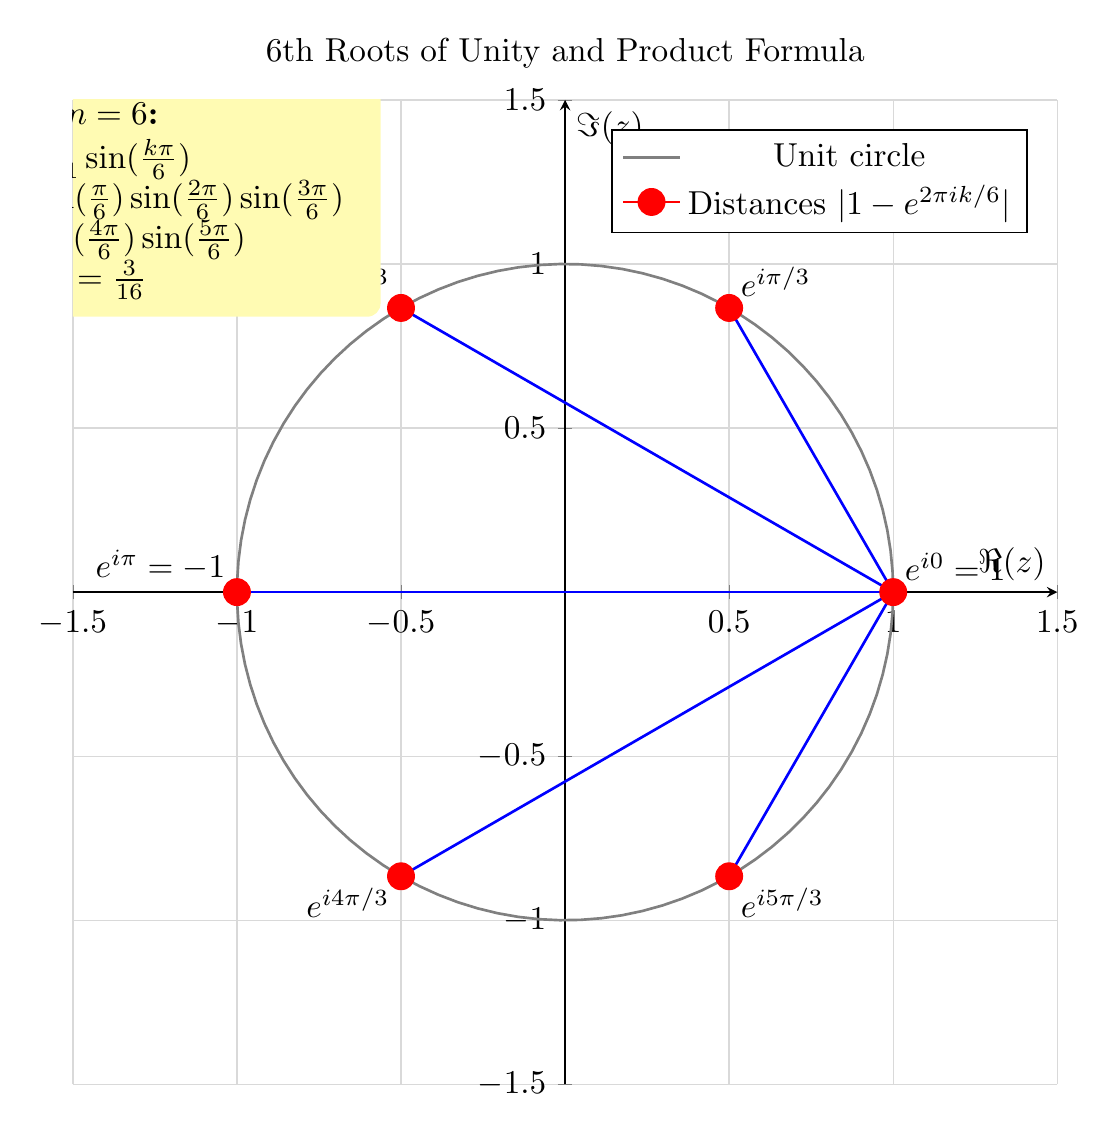
\begin{tikzpicture}[scale=1.2]
\begin{axis}[
    width=12cm,
    height=12cm,
    xlabel={$\Re(z)$},
    ylabel={$\Im(z)$},
    title={6th Roots of Unity and Product Formula},
    xmin=-1.5, xmax=1.5,
    ymin=-1.5, ymax=1.5,
    grid=major,
    grid style={gray!30},
    axis lines=middle,
    axis equal,
    legend pos=north east
]

% Unit circle
\addplot[gray, thick, samples=100, domain=0:360] ({cos(x)}, {sin(x)});
\addlegendentry{Unit circle}

% 6th roots of unity
\addplot[red, mark=*, mark size=4pt] coordinates {(1,0)};
\node[above right] at (axis cs:1,0) {$e^{i0} = 1$};

\addplot[red, mark=*, mark size=4pt] coordinates {(0.5,0.866)};
\node[above right] at (axis cs:0.5,0.866) {$e^{i\pi/3}$};

\addplot[red, mark=*, mark size=4pt] coordinates {(-0.5,0.866)};
\node[above left] at (axis cs:-0.5,0.866) {$e^{i2\pi/3}$};

\addplot[red, mark=*, mark size=4pt] coordinates {(-1,0)};
\node[above left] at (axis cs:-1,0) {$e^{i\pi} = -1$};

\addplot[red, mark=*, mark size=4pt] coordinates {(-0.5,-0.866)};
\node[below left] at (axis cs:-0.5,-0.866) {$e^{i4\pi/3}$};

\addplot[red, mark=*, mark size=4pt] coordinates {(0.5,-0.866)};
\node[below right] at (axis cs:0.5,-0.866) {$e^{i5\pi/3}$};

% Show the distances from 1 to other roots
\addplot[blue, thick, ->] coordinates {(1,0) (0.5,0.866)};
\addplot[blue, thick, ->] coordinates {(1,0) (-0.5,0.866)};
\addplot[blue, thick, ->] coordinates {(1,0) (-1,0)};
\addplot[blue, thick, ->] coordinates {(1,0) (-0.5,-0.866)};
\addplot[blue, thick, ->] coordinates {(1,0) (0.5,-0.866)};
\addlegendentry{Distances $|1 - e^{2\pi i k/6}|$}

% Add text showing the product
\node[fill=yellow!30, rounded corners, inner sep=5pt] at (axis cs:-1.2,1.2) {
    \begin{tabular}{l}
    \textbf{For $n = 6$:} \\
    $\prod_{k=1}^5 \sin(\frac{k\pi}{6})$ \\
    $= \sin(\frac{\pi}{6}) \sin(\frac{2\pi}{6}) \sin(\frac{3\pi}{6})$ \\
    $\quad \sin(\frac{4\pi}{6}) \sin(\frac{5\pi}{6})$ \\
    $= \frac{6}{2^5} = \frac{3}{16}$
    \end{tabular}
};

\end{axis}
\end{tikzpicture}
\end{center}

This visualization shows the 6th roots of unity on the unit circle. The blue arrows show the distances from $z = 1$ to the other roots, which are related to the sine values in the product formula. For $n = 6$, the product equals $\frac{6}{2^5} = \frac{3}{16}$.

\section{Solving and Proving Techniques}

\subsection*{Proving by Contradiction}
\begin{enumerate}
\item Assume the opposite of what you want to prove
\item Show this leads to a logical contradiction
\item Conclude the original statement must be true
\end{enumerate}
Used in Problems 1.1, 1.9, 1.14, 1.16, 1.17, 1.18, 1.20, 1.22

\subsection*{Mathematical Induction}
\begin{enumerate}
\item Verify the base case (usually $n = 1$)
\item Assume the statement holds for $n = k$ (inductive hypothesis)
\item Prove it holds for $n = k + 1$ using the hypothesis
\item Conclude it holds for all positive integers
\end{enumerate}
Used in Problem 1.5 with strong induction

\subsection*{Proving Irrationality}
\begin{enumerate}
\item Assume the number is rational (express as $\frac{p}{q}$)
\item Square both sides to eliminate square roots
\item Show this leads to a contradiction (usually that a prime divides both numerator and denominator)
\end{enumerate}
Used in Problems 1.9, 1.14

\subsection*{Finding Supremum and Infimum}
\begin{enumerate}
\item For finite sets: find maximum and minimum values
\item For intervals: use the endpoints
\item For infinite sets: analyze limiting behavior
\item For sets defined by inequalities: solve the inequalities to find bounds
\end{enumerate}
Used in Problems 1.19, 1.20, 1.21

\subsection*{Proving Inequalities}
\begin{itemize}
\item Use known inequalities (Triangle, Cauchy-Schwarz, etc.)
\item Complete the square or use algebraic manipulation
\item Consider cases based on signs of variables
\item Use the fact that squares are non-negative
\item Used in Problems 1.24, 1.25, 1.26, 1.32, 1.33, 1.48
\end{itemize}

\subsection*{Working with Complex Numbers}
\begin{itemize}
\item Use $i^2 = -1$ and powers of $i$ cycle every 4
\item For division, multiply numerator and denominator by complex conjugate
\item Use $|z|^2 = z \cdot \overline{z}$ and $\arg(z) = \tan^{-1}(\frac{y}{x})$ (with quadrant adjustments)
\item Use De Moivre's theorem: $(\cos \theta + i \sin \theta)^n = \cos(n\theta) + i \sin(n\theta)$
\item Used in Problems 1.27, 1.28, 1.29, 1.30, 1.31, 1.32, 1.33, 1.34, 1.35, 1.36, 1.37, 1.38, 1.39, 1.40, 1.41, 1.42, 1.43, 1.44, 1.45, 1.46, 1.47, 1.48, 1.49, 1.50
\end{itemize}

\subsection*{Proving Uniqueness}
\begin{enumerate}
\item Assume two different objects satisfy the same conditions
\item Show they must actually be equal
\item Often use contradiction or direct comparison
\end{enumerate}
Used in Problems 1.17, 1.18

\subsection*{Using the Pigeonhole Principle}
\begin{enumerate}
\item Divide a set into fewer subsets than elements
\item Show at least one subset must contain multiple elements
\item Use this to find numbers that are close together
\end{enumerate}
Used in Problem 1.15

\subsection*{Proving Existence}
\begin{enumerate}
\item Construct an explicit example
\item Use intermediate value theorem or similar existence results
\item Show that assuming non-existence leads to contradiction
\end{enumerate}
Used in Problems 1.11, 1.15, 1.16

\subsection*{Working with Series and Sums}
\begin{itemize}
\item Use telescoping series where terms cancel
\item Apply geometric series formulas
\item Use binomial theorem for expansions
\item Factor polynomials and use partial fractions
\item Used in Problems 1.2, 1.17, 1.40, 1.49, 1.50
\end{itemize}

\subsection*{Proving Geometric Properties}
\begin{itemize}
\item Use coordinate geometry and distance formulas
\item Apply properties of circles, lines, and triangles
\item Use complex numbers to represent geometric objects
\item Show that conditions imply specific geometric configurations
\item Used in Problems 1.13, 1.30, 1.31, 1.34
\end{itemize}

\subsection*{Using Trigonometric Identities}
\begin{itemize}
\item Apply double angle, sum, and difference formulas
\item Use De Moivre's theorem to derive new identities
\item Express complex functions in terms of real and imaginary parts
\item Use periodicity and symmetry properties
\item Used in Problems 1.44, 1.45, 1.46, 1.47, 1.49, 1.50
\end{itemize}

\subsection*{Proving Ordering Properties}
\begin{enumerate}
\item Check trichotomy (exactly one of $a < b$, $a = b$, $a > b$ holds)
\item Verify transitivity ($a < b$ and $b < c$ implies $a < c$)
\item Test invariance under operations (addition, multiplication)
\item Provide counterexamples when axioms fail
\end{enumerate}
Used in Problems 1.36, 1.37

\subsection*{Working with Logarithms and Exponentials}
\begin{itemize}
\item Use $\log(ab) = \log a + \log b$ and $\log(a^b) = b \log a$
\item Remember that complex logarithms have multiple branches
\item Use $e^{i\theta} = \cos \theta + i \sin \theta$ for complex exponentials
\item Apply properties of complex powers carefully
\item Used in Problems 1.38, 1.39, 1.41, 1.42, 1.43
\end{itemize}

\subsection*{Proving Polynomial Identities}
\begin{itemize}
\item Expand both sides and show they are equal
\item Use roots of unity and factorization
\item Apply Vieta's formulas to relate coefficients to roots
\item Use polynomial division and remainder theorem
\item Used in Problems 1.23, 1.40, 1.49, 1.50
\end{itemize}
